\documentclass[spanish]{thesis}

\author{Ruslan Alexei Martinez Campos}
\title{Videojuego educativo para la enseñanza de los Objetivos de Desarrollo Sostenible}
\ucicenter{Facultad de Tecnologías Interactivas}
\facultynum{4}
\addtutor{P.T., Ing. Juan Antonio Plasencia Soler, Dr. C.}
\addtutor{Ing. Oscar de Jesús Pacheco del Pino}

\thought{``El juego es la forma más elevada de investigación''\\
 Albert Einstein}
 
\dedicatory{A mi madre, por ser el pilar inquebrantable de mi vida y mi mayor certeza. Todo tu amor infinito, sacrificio y apoyo incondicional han sido el verdadero motor que me impulsó a no rendirme y a superar cada reto a lo largo de mi formación como ingeniero. Este logro es tan tuyo como mío.}

\acknowledgment{A mi familia, por ser mi refugio constante. En especial a mi papá, por siempre iluminarme con su sabiduría y brindarme su conocimiento. A mi abuela y a mi tía, por su apoyo diario, paciente y eterno, que me sostuvo a lo largo de este camino.

A mi pareja, por ser mi gran pilar, apoyándome con la misma fuerza e intensidad tanto en la distancia como cuando hemos estado juntos.

A mis amigos de la vida, y muy en especial a José Miguel, Yoel, Yslen y Óscar, por ayudarme a orientarme y por su invaluable apoyo durante todo este largo proceso.

A mi otra familia forjada en estos cuatro intensos años. Gracias por hacer de esta etapa un recuerdo inolvidable a través de todos los incontables momentos compartidos durante nuestra convivencia en el entrañable 83 204.

Por último, deseo extender mi más profunda gratitud a mi tutor, por confiar en mí y darme la excepcional oportunidad de desarrollar un ejercicio de culminación de estudios enfocado en materializar y explorar lo que realmente me apasiona.}

\abstract{El desconocimiento generalizado sobre los Objetivos de Desarrollo Sostenible (ODS) de las Naciones Unidas dificulta la participación activa en la Agenda 2030 y limita la toma de decisiones informadas. Promover un conocimiento profundo de estos 17 objetivos es crucial para mejorar la calidad de vida y fomentar el desarrollo equitativo. En este contexto, los videojuegos educativos, especialmente aquellos basados en simulación y Aprendizaje Basado en Juegos (ABJ), emergen como una herramienta eficaz, generando experiencias inmersivas que facilitan el aprendizaje significativo gracias a su capacidad para integrar narrativas y retroalimentación inmediata. El presente documento describe el proceso completo de desarrollo de una solución basada en videojuegos, siguiendo la metodología Extreme Programming (XP) en sus fases de planificación, diseño e implementación. Dicho proceso abarcó desde la selección del motor de videojuegos (Godot) y la obtención rigurosa de requisitos funcionales y no funcionales de software mediante historias de usuario, hasta el diseño de interfaces, la construcción de una arquitectura escalable y la implementación de componentes esenciales (tablero, preguntas, mecanismos de avance). Como resultado de la aplicación de esta metodología se obtuvo el videojuego educativo \textit{Go Goals! Digital}. Finalmente, la aplicación de pruebas de software, en particular las pruebas de aceptación, permitió validar la calidad y eficacia de la solución propuesta.}{The widespread lack of knowledge about the United Nations' Sustainable Development Goals (SDGs) limits public engagement with the 2030 Agenda and hinders informed decision-making. Promoting a deeper understanding of the 17 goals is crucial for improving quality of life and fostering equitable development. In this context, educational video games, especially those based on simulation and Game-Based Learning (GBL), emerge as an effective tool, offering immersive experiences that support meaningful learning by integrating strong narratives and immediate feedback. This document outlines the complete development process of a video-game-based solution, following the Extreme Programming (XP) methodology through its planning, design, and implementation phases. This process ranged from the selection of the game engine (Godot) and the rigorous gathering of functional and non-functional software requirements through user stories, to the design of graphical interfaces and the establishment of a scalable software architecture. Key game components are described, and as a result of applying this methodology, the educational video game \textit{Go Goals! Digital} was obtained. Finally, the execution of software testing, particularly acceptance tests, validated the proposed solution's quality and effectiveness.}

\keywords{Agenda 2030, Aprendizaje Basado en Juegos, Godot Engine, ODS, videojuegos educativos}

\keywordsen{2030 Agenda, educational video games, Game-Based Learning, Godot Engine, SDGs}

\newglossaryentry{Engine}{name={Motor de Videojuegos}, description={Sistema de software diseñado para la creación y desarrollo de videojuegos}}
\newglossaryentry{GDScript}{name={GDScript}, description={Lenguaje de programación de alto nivel, tipado dinámico y optimizado para el motor Godot}}
\newglossaryentry{Autoload}{name={Autoload}, description={Nodos que se cargan automáticamente al inicio del juego y son accesibles globalmente (Singletons)}}
\newglossaryentry{Tween}{name={Tween}, description={Interpolación de valores para crear animaciones fluidas por código}}
\newglossaryentry{SVG}{name={SVG}, description={Gráficos Vectoriales Redimensionables, formato de imagen vectorial para elementos escalables}}
\newglossaryentry{Snapshot}{name={Snapshot}, description={Instantánea del estado de un sistema en un momento determinado, utilizada por Git para el control de versiones}}
\newacronym{UCI}{UCI}{Universidad de las Ciencias Informáticas}
\newacronymeng{SCADA}{SCADA}{Supervisión, Control y Adquisición de Datos}


\addbibresource{example.bib}

\usepackage{float}

\begin{document}
  \maketitle
  
  \introduction

La sostenibilidad se define como la capacidad de satisfacer las necesidades del presente sin comprometer la capacidad de las futuras generaciones para satisfacer sus propias demandas, abarcando la interrelación entre el desarrollo económico, la inclusión social y la protección del medio ambiente \parencite{WCED1987}. Este concepto implica un enfoque holístico que busca un equilibrio entre estos tres pilares para garantizar un futuro viable para todos. Las dimensiones de la sostenibilidad se dividen comúnmente en tres categorías principales: la dimensión económica, centrada en el crecimiento y la eficiencia de recursos a largo plazo \parencite{Stiglitz2018}; la dimensión social, que promueve la equidad, la inclusión y el bienestar humano \parencite{NacionesUnidas2015}; y la dimensión ambiental, enfocada en la conservación de la biodiversidad y la gestión responsable de los recursos naturales \parencite{EuropeanUnion2024}.

La educación para el desarrollo sostenible es fundamental en la promoción de un futuro equitativo. Este tipo de educación no solo busca transmitir conocimientos, sino que también fomenta habilidades y actitudes que permiten a las personas tomar decisiones informadas y responsables. La Educación para el Desarrollo Sostenible (EDS) es un enfoque integral que empodera a los ciudadanos para participar activamente en la construcción de sociedades justas y sostenibles \parencite{UNESCO2017, UNESCO2020EDS}. Además, la EDS contribuye directamente a la consecución de los Objetivos de Desarrollo Sostenible (ODS), especialmente a la meta 4.7 del ODS 4, garantizando que las personas adquieran los conocimientos teóricos y prácticos necesarios para promover estilos de vida sostenibles \parencite{NacionesUnidas2015, UNESCO2020EDS}.

La educación es un derecho humano fundamental y un motor clave para el desarrollo sostenible. Sin embargo, persisten brechas críticas: en 2021, 244 millones de niños y jóvenes estaban sin escolarizar, cifra que refleja desigualdades arraigadas en geografía y nivel socioeconómico \parencite{GlobalEduReport2022}. Estas brechas se intensifican en crisis humanitarias y se ven exacerbadas por fenómenos globales que limitan el acceso a la educación a distancia \parencite{UNICEF2020}. En América Latina, la falta de dispositivos y conectividad afecta significativamente la continuidad educativa \parencite{BancoMundial2025}. Por ello, abordar estas brechas resulta esencial para lograr una educación inclusiva, equitativa y de calidad para todos.

En Cuba, el sistema educativo constituye históricamente un pilar del desarrollo social. El 99{,}7\% de su población adulta está alfabetizada \parencite{UNESCO2023}, y la educación es gratuita en todos los niveles tal como lo establece la Constitución de la República \parencite{CubaConstitucion2019}. En el panorama nacional, el desarrollo guiado por ingeniería formal de software interactivo para los ODS discurre en su fase embrionaria, aunque cimentado en proyecciones tecnológicas provenientes del ámbito universitario y apuestas sólidas como el plan de informatización escolar Aula Digital. El archipiélago orienta gradualmente el perfeccionamiento continuo del capital lúdico digital introducido a las aulas de educación básica escolarizada \parencite{InformeVoluntarioCuba2021}. No obstante, persisten desafíos como la escasez de materiales didácticos digitales, la obsolescencia tecnológica y las limitaciones de conectividad que afectan la calidad educativa. Las fluctuaciones de suministro en el ecosistema físico acentúan un rezago en la disponibilidad masiva de periféricos de última línea, mermando el campo efectivo de las iniciativas puramente conectadas y exigiendo arquitecturas optimizadas \parencite{BancoMundial2023, MesaLago2022}.

Los videojuegos se posicionan como herramientas pedagógicas innovadoras para abordar desafíos de sostenibilidad. Desde una perspectiva histórica, los juegos de mesa constituyen herramientas pedagógicas por excelencia durante siglos, ofreciendo entornos estructurados donde los participantes desarrollan habilidades cognitivas, sociales y estratégicas de manera lúdica. La digitalización de estos juegos representa una evolución natural que mantiene la esencia pedagógica del formato original mientras amplifica sus posibilidades mediante la interactividad digital, la retroalimentación inmediata y la eliminación de barreras logísticas \parencite{MartinezGimenes2023}. Esta transición del formato físico al digital no implica una simple traslación de mecánicas, sino una reconfiguración que aprovecha las capacidades computacionales para enriquecer la experiencia de aprendizaje.

En el ámbito internacional, las Naciones Unidas desarrollan el juego de mesa \textit{Go Goals!} como herramienta pedagógica oficial para introducir los diecisiete ODS a niños de entre ocho y diez años \parencite{GoGoals2020}. Este juego utiliza una estructura inspirada en el clásico Serpientes y Escaleras, adaptando sus mecánicas tradicionales para incorporar contenidos educativos específicos sobre sostenibilidad mediante un sistema de preguntas y respuestas que refuerzan el aprendizaje. Su simplicidad y familiaridad facilitan la comprensión de las reglas, permitiendo que el foco cognitivo se centre en el contenido educativo.

El conocimiento de los ODS conlleva múltiples beneficios: alineación con la Agenda Global, mejora en la toma de decisiones y fomento de la responsabilidad social y ambiental \parencite{R3crea2022}. Por el contrario, su desconocimiento genera desalineación con tendencias internacionales, uso inadecuado de recursos y menor preparación para enfrentar desafíos globales como el cambio climático \parencite{EcologiaVerde2024}.

A pesar de su reconocimiento internacional, el formato físico del juego \textit{Go Goals!} presenta limitaciones estructurales inherentes que restringen su acceso, escalabilidad, rejugabilidad y capacidad de evaluación del aprendizaje. A esto se suma que la adaptación digital específica de juegos de mesa reconocidos internacionalmente como \textit{Go Goals!} representa un vacío identificado en la oferta actual de recursos educativos tecnológicos en Cuba. No se documenta la existencia de un videojuego desarrollado en el país que se centre exclusivamente en la enseñanza de los ODS mediante esta mecánica lúdica particular. Esta ausencia evidencia una brecha digital significativa considerando la creciente asimilación de los videojuegos en el público joven y su demostrada capacidad para facilitar el Aprendizaje Basado en Juegos. Aprovechando el potencial pedagógico de los videojuegos educativos y la estructura probada del juego de mesa original, se identifica la necesidad de desarrollar una versión digital que supere las barreras del formato físico y mitigue esta brecha en el contexto educativo.

A partir de la situación problemática antes expuesta, se plantea como problema de la investigación: ¿Cómo contribuir a la enseñanza de los Objetivos de Desarrollo Sostenible? Como objeto de estudio se tienen los videojuegos educativos como herramientas para la promoción de los ODS, enmarcados en el campo de acción: el proceso de desarrollo de un videojuego educativo basado en la adaptación digital del juego de mesa \textit{Go Goals!}. El objetivo general es desarrollar un videojuego educativo basado en la adaptación digital del juego de mesa \textit{Go Goals!} que contribuya a la promoción de los Objetivos de Desarrollo Sostenible.

\subsection*{Tareas de la investigación}

\begin{itemize}
    \item Sistematización de los referentes teóricos y metodológicos que sustentan el uso de videojuegos educativos para la promoción de los Objetivos de Desarrollo Sostenible.
    \item Análisis de soluciones homólogas y diagnóstico del estado actual del juego analógico \textit{Go Goals!} para determinar los elementos susceptibles de informatización.
    \item Selección de las tecnologías, herramientas y metodologías idóneas para la implementación del sistema.
    \item Elaboración del diseño arquitectónico, definición de mecánicas y especificación de requisitos funcionales y no funcionales del videojuego.
    \item Implementación del videojuego educativo a partir de la adaptación digital del referente analógico seleccionado.
    \item Validación del sistema mediante la ejecución de pruebas de calidad de software que avalan su despliegue y pertinencia.
\end{itemize}

\subsection*{Métodos teóricos de investigación}

Los métodos teóricos de investigación resultan esenciales para explorar y comprender fenómenos complejos en distintas disciplinas académicas. Permiten analizar, interpretar y sintetizar teorías y conceptos, fomentando el avance del conocimiento y la generación de nuevas perspectivas. A través del análisis conceptual, la revisión bibliográfica y la síntesis teórica, los investigadores profundizan en las bases teóricas de sus estudios, estableciendo conexiones significativas entre ideas y enfoques diversos. Estos métodos no solo fundamentan la investigación, sino que también contribuyen a la construcción de conocimiento sólido en el ámbito académico.

Analítico-sintético: se utiliza para extraer las ideas fundamentales que respaldan teóricamente la investigación y la propuesta presentada. Este enfoque se justifica debido a la necesidad de establecer una base sólida y coherente para el estudio, asegurando que las ideas esenciales sean identificadas y comprensiblemente integradas en el marco teórico. La revisión exhaustiva de la literatura existente permite situar el estudio dentro del contexto académico pertinente, proporcionando un fundamento robusto para el desarrollo y la argumentación de la investigación propuesta.

Modelación: constituye una herramienta esencial en la investigación, adoptando formas tanto tangibles como abstractas, con el propósito de replicar y comprender a fondo el objeto de estudio. Funciona como una representación concreta o conceptual de un fenómeno o proceso, permitiendo una mayor claridad en la comprensión de sus características, desarrollo y funcionamiento. A través de esquemas, diagramas o representaciones, se capturan las interrelaciones y propiedades clave de la realidad, facilitando así la exploración y el análisis detallado de la materia investigada.

\subsection*{Métodos empíricos}

Los métodos empíricos en la investigación constituyen un enfoque fundamental que se basa en la observación y la experiencia directa para obtener datos y validar hipótesis. Estos métodos implican la recopilación sistemática de información a través de la experimentación, la observación o la recolección de datos cuantitativos y cualitativos en el entorno real. Al emplear métodos empíricos, los investigadores pueden poner a prueba teorías, validar resultados y generar conocimiento sustentado en evidencia concreta y verificable.

Observación: se emplea para analizar soluciones homólogas existentes en el ámbito de los videojuegos educativos sobre sostenibilidad, identificando características, mecánicas de juego y enfoques pedagógicos que informan el diseño de la solución propuesta.

Entrevista: facilita una comprensión más profunda de los requerimientos del cliente al interactuar con la aplicación. Esto ayuda a recopilar información directamente del cliente y, durante la fase de pruebas, a evaluar su satisfacción con los resultados obtenidos.

\subsection*{Estructura capitular}

\textbf{Capítulo 1}: Fundamentación teórica, en el cual se examinan en detalle los conceptos fundamentales que comprenden el marco teórico de la investigación. Se ahonda, además, en el ámbito de los videojuegos educativos y sus características. También se estudian soluciones homólogas para establecer comparaciones. Asimismo, se exploran las herramientas, tecnologías que se emplean para el desarrollo del sistema y las metodologías de desarrollo de software.

\textbf{Capítulo 2}: Diseño e implementación, donde se detalla la propuesta de solución a través de la metodología de desarrollo de software seleccionada. Se definen los requisitos funcionales y no funcionales del sistema y se detallan las interfaces de usuario y tarjetas CRC para documentar la parte visual del proyecto y estructurar la arquitectura de la solución.

\textbf{Capítulo 3}: Resultados y validación, en el que se documentan los resultados de las pruebas realizadas en el despliegue de la solución.

  \chapter{Fundamentos y referentes teórico-metodológicos sobre el objeto de estudio}
\label{chap:chapter1}

El presente capítulo tiene como objetivo sistematizar los fundamentos teórico-metodológicos que sustentan el desarrollo de un videojuego educativo para la promoción de los Objetivos de Desarrollo Sostenible. Se aborda, en primer lugar, el marco conceptual de los videojuegos educativos y el aprendizaje basado en juegos; en segundo lugar, se analizan los antecedentes de la gamificación aplicada a la educación para el desarrollo sostenible; en tercer lugar, se describe y diagnostica el estado actual del juego de mesa ``Go Goals!'' como objeto de estudio; y finalmente, se justifican las tecnologías y herramientas seleccionadas para la implementación de la solución propuesta. El capítulo cierra con las conclusiones que fundamentan las decisiones adoptadas en la investigación.

\section{Fundamentos teóricos de los videojuegos educativos}

El presente epígrafe sistematiza los principios teóricos y metodológicos que sustentan la incorporación de videojuegos educativos como recursos de aprendizaje significativo, especialmente cuando se diseñan a partir de dinámicas lúdicas tradicionales como los juegos de mesa y se orientan a la enseñanza de conceptos vinculados con la sostenibilidad. Su objetivo es establecer el marco conceptual que fundamenta la pertinencia pedagógica de la propuesta desarrollada en esta investigación.

\subsection{Antecedentes del aprendizaje mediante el juego}
La utilización del juego en la educación posee una sólida tradición teórica. El juego se reconoce como un medio natural para el desarrollo cognitivo, pues permite interactuar con reglas, roles y condiciones simbólicas que estimulan la construcción activa de estructuras mentales. Esta perspectiva se complementa con el enfoque sociocultural, según el cual el juego posibilita niveles superiores de desempeño cognitivo y social mediante la mediación y la interacción significativa. En el campo educativo contemporáneo, estos aportes han evolucionado hacia enfoques que consideran el juego no solo como actividad recreativa, sino como un entorno estructurado donde el aprendizaje ocurre de manera contextualizada, motivante y autónoma.

\subsection{Fundamentos del Aprendizaje Basado en Juegos (Game-Based Learning)}
El Aprendizaje Basado en Juegos (GBL) se define como la integración sistemática de mecánicas, reglas y dinámicas propias de los juegos dentro del proceso de enseñanza. Los entornos lúdicos proporcionan condiciones particularmente fértiles para la adquisición de conocimientos y el desarrollo de habilidades cognitivas superiores, al permitir la interacción significativa con los contenidos, la toma de decisiones dentro de escenarios estructurados, la retroalimentación inmediata y el aprendizaje situado en contextos simulados. Estos elementos convierten a los juegos analógicos o digitales en plataformas eficaces para introducir conceptos complejos como los Objetivos de Desarrollo Sostenible, la acción climática o la gestión responsable de recursos.

\subsection{Gamificación como estrategia educativa}
La gamificación constituye un enfoque complementario, centrado en la incorporación de elementos característicos de los juegos ---puntos, retroalimentación inmediata, progresión, niveles y desafíos--- dentro de situaciones originalmente no lúdicas. En el ámbito educativo, esta estrategia se asocia a incrementos en la motivación intrínseca, la participación activa del estudiantado, la claridad en las metas del aprendizaje y la percepción de logro y autonomía. El uso de mecánicas gamificadas resulta especialmente relevante en recursos formativos vinculados con la sostenibilidad, donde la motivación y el compromiso con la acción son tan importantes como el conocimiento conceptual.

\subsection{Enfoques metodológicos relevantes para el diseño educativo digital}
El diseño y análisis de videojuegos con fines educativos requiere integrar modelos que articulen los aspectos pedagógicos, tecnológicos y disciplinares. Dos marcos metodológicos resultan especialmente relevantes. La Teoría del flujo explica cómo los entornos lúdicos mantienen la motivación cuando existe equilibrio entre el desafío y la habilidad del jugador; esta teoría orienta la organización del ritmo, la dificultad y la retroalimentación dentro del juego. El Modelo TPACK (Tecnológico-Pedagógico-Disciplinar) proporciona un marco para integrar contenido educativo, estrategias pedagógicas y decisiones tecnológicas, permitiendo evaluar la coherencia entre las mecánicas de juego, los objetivos formativos y los recursos digitales seleccionados.

\section{Gamificación en la educación para el desarrollo sostenible}

Los videojuegos educativos basados en adaptaciones de juegos de mesa constituyen una categoría especializada que combina la accesibilidad y las mecánicas probadas del formato analógico con las capacidades tecnológicas del medio digital. El presente epígrafe sistematiza los fundamentos teórico-metodológicos asociados a este tipo de desarrollo, específicamente la adaptación digital de juegos de mesa educativos como herramientas para promover los Objetivos de Desarrollo Sostenible, estableciendo los referentes que sustentan la investigación tanto en el contexto internacional como nacional.

Desde una perspectiva histórica, los juegos de mesa han constituido herramientas pedagógicas por excelencia durante siglos, ofreciendo entornos estructurados donde los participantes desarrollan habilidades cognitivas, sociales y estratégicas de manera lúdica. La digitalización de estos juegos representa una evolución natural que mantiene la esencia pedagógica del formato original mientras amplifica sus posibilidades mediante la interactividad digital, la retroalimentación inmediata y la eliminación de barreras logísticas.

En el ámbito internacional, las Naciones Unidas desarrollaron el juego de mesa Go Goals! como herramienta pedagógica oficial para introducir los diecisiete Objetivos de Desarrollo Sostenible a niños de 8 a 10 años. Este juego utiliza una estructura inspirada en el clásico Serpientes y Escaleras, adaptando sus mecánicas tradicionales para incorporar contenidos educativos específicos sobre sostenibilidad mediante un sistema de preguntas y respuestas que refuerzan el aprendizaje de cada objetivo.

La estructura pedagógica de Go Goals! se fundamenta en principios de gamificación aplicados a contextos educativos. El juego emplea un tablero de 63 casillas hexagonales que representan el recorrido temporal desde el presente hasta el año 2030, horizonte establecido por la Agenda 2030. Esta metáfora visual del progreso temporal refuerza la comprensión de que la sostenibilidad es un proceso continuo que requiere acciones sostenidas en el tiempo. El tablero incorpora diecisiete casillas temáticas, una por cada ODS, donde los jugadores deben responder preguntas específicas para avanzar.

\begin{table}[!htbp]
\centering
\caption{Ejemplos de preguntas por nivel cognitivo según ODS\label{tab:preguntas_niveles}}
\begin{tabular}{|p{0.2\textwidth}|p{0.35\textwidth}|p{0.35\textwidth}|}
\hline
\textbf{ODS} & \textbf{Pregunta nivel bajo (comprensión)} & \textbf{Pregunta nivel alto (aplicación / análisis)} \\
\hline
1. Fin de la pobreza & ¿Cómo definir la pobreza? $\rightarrow$ No puede costear necesidades básicas & ¿La pobreza mundial ha disminuido en 25 años? $\rightarrow$ Sí, 1000 millones han salido de la pobreza \\
\hline
6. Agua limpia y saneamiento & ¿Qué es el agua potable? $\rightarrow$ Agua segura de beber & ¿Cómo ahorrar agua en casa? $\rightarrow$ Duchándote en vez de bañarte \\
\hline
13. Acción por el clima & ¿Qué es energía renovable? $\rightarrow$ Energía de recursos que se renuevan rápido & ¿Por qué proteger los bosques? $\rightarrow$ Producen oxígeno \\
\hline
\end{tabular}
\end{table}

En el ámbito de la educación para el desarrollo sostenible, videojuegos como Eco (simulación de ecosistemas) y Fate of the World (políticas climáticas globales) demuestran cómo las herramientas digitales transforman información abstracta en experiencias concretas que fomentan la comprensión sistémica de las dimensiones económica, social y ambiental. A nivel nacional, aunque el desarrollo de videojuegos educativos orientados a los ODS se encuentra en fase incipiente, existen antecedentes valiosos en programas como Aula Digital y diversas iniciativas universitarias. Sin embargo, la adaptación digital específica de juegos de mesa reconocidos internacionalmente como Go Goals! representa un vacío identificado en la oferta actual de recursos educativos tecnológicos, especialmente en la Universidad de las Ciencias Informáticas.

\section{Análisis del estado actual del juego de mesa Go Goals!}

El presente epígrafe se dedica a la descripción y análisis exhaustivo del estado actual del objeto de estudio, el juego de mesa Go Goals! en su formato físico original, estableciendo claridad sobre las variables que se estudian y presentando los resultados del diagnóstico realizado previo al inicio de la investigación. Este análisis demuestra la pertinencia de la investigación y valida tanto la situación problemática como el problema científico planteado.

\subsection{Descripción del juego Go Goals! en su formato original}
El juego de mesa Go Goals! constituye un recurso educativo oficial desarrollado por las Naciones Unidas con el propósito específico de introducir los diecisiete Objetivos de Desarrollo Sostenible a poblaciones infantiles de manera lúdica y accesible. Dirigido específicamente a niños de ocho a diez años, el juego busca promover el aprendizaje activo, la interacción social y la motivación por la acción sostenible mediante mecánicas de juego probadas que han demostrado efectividad pedagógica durante décadas. Su estructura se basa en el clásico juego Serpientes y Escaleras, adaptado para incorporar contenidos educativos específicos sobre cada uno de los ODS mediante un sistema integrado de preguntas y respuestas.

\begin{table}[!htbp]
\centering
\caption{Componentes del juego de mesa Go Goals!\label{tab:componentes_juego}}
\begin{tabular}{|l|p{0.7\textwidth}|}
\hline
\textbf{Componente} & \textbf{Descripción} \\
\hline
Tablero & 63 casillas hexagonales conectadas en un recorrido no lineal. Incluye 17 casillas temáticas (una por ODS), escaleras (avance positivo) y serpientes (retroceso correctivo). \\
\hline
Fichas de jugadores & 6 fichas personalizables con el personaje Elyx (mascota oficial de la ONU). \\
\hline
Dado & Un dado de 6 caras para determinar el avance aleatorio. \\
\hline
Cartas de preguntas & 34 cartas (2 por ODS), con preguntas de opción múltiple, verdadero/falso y selección múltiple. \\
\hline
Instrucciones & Reglas completas en español, inglés y otros idiomas. \\
\hline
\end{tabular}
\end{table}

\subsection{Diagnóstico: fortalezas y limitaciones}
Un análisis riguroso del juego en su formato físico actual revela tanto fortalezas significativas como limitaciones críticas que justifican la necesidad de una adaptación digital. Las fortalezas incluyen un alto valor pedagógico con mecánicas probadas, lenguaje accesible para el grupo de edad objetivo y una progresión cognitiva según la taxonomía de Bloom. Entre las limitaciones más relevantes se destacan el contenido estático derivado de solo 34 preguntas fijas, la dependencia de recursos de impresión a color, la imposibilidad de uso en entornos de educación a distancia y la ausencia de mecanismos de registro del aprendizaje individual.

\begin{table}[!htbp]
\centering
\caption{Diagnóstico del estado actual de Go Goals! (formato físico)\label{tab:diagnostico}}
\begin{tabular}{|p{0.2\textwidth}|p{0.35\textwidth}|p{0.35\textwidth}|}
\hline
\textbf{Aspecto} & \textbf{Fortalezas} & \textbf{Limitaciones} \\
\hline
Diseño pedagógico & Alta alineación con ODS, mecánicas probadas durante décadas, lenguaje accesible para 8-10 años. & Contenido estático: solo 34 preguntas fijas. Rejugabilidad limitada por memorización. \\
\hline
Interacción social & Fomenta cooperación, genera discusión sobre sostenibilidad, enseña respeto de turnos. & Requiere grupo físico y materiales impresos. Imposible en educación a distancia. \\
\hline
Accesibilidad & Gratuito, multilingüe, formato imprimible disponible en portal oficial de la ONU. & Dependiente de impresora a color; inaccesible en zonas rurales o de bajos recursos. \\
\hline
Escalabilidad & Ideal para aulas pequeñas (4-6 jugadores) con recursos adecuados. & Imposible jugar en línea o con grupos grandes. No permite distribución masiva. \\
\hline
Medición del aprendizaje & Retroalimentación cualitativa inmediata (respuesta correcta $\rightarrow$ avance). & Sin registro de progreso longitudinal ni evaluación cuantitativa. \\
\hline
\end{tabular}
\end{table}

La adaptación digital propuesta mediante Godot Engine resuelve estas limitaciones al ofrecer acceso universal mediante descarga gratuita en múltiples plataformas, un banco de preguntas ampliable mediante archivos de datos estructurados, registro automático del progreso y patrones de aprendizaje, y una experiencia enriquecida con animaciones, sonido y efectos visuales. La situación problemática identificada puede caracterizarse como un recurso educativo de alto valor pedagógico cuyo alcance e impacto potencial se ven severamente limitados por restricciones inherentes a su formato analógico.

\section{Tecnologías y herramientas para el desarrollo del videojuego educativo}

El presente epígrafe se dedica a la sistematización de los fundamentos teórico-metodológicos asociados a las tecnologías y herramientas utilizadas para lograr el resultado contenido en el campo de acción, es decir, la adaptación digital del juego de mesa ``Go Goals!'' mediante un videojuego educativo interactivo. Se analizan y justifican la metodología de desarrollo, el motor de videojuegos, los lenguajes de programación y modelado, así como las herramientas de soporte seleccionadas.

\subsection{Metodología de desarrollo de software: Extreme Programming}
Una metodología de desarrollo de software es un conjunto de principios, prácticas y procesos sistemáticos que guían la planificación, diseño, implementación, prueba y mantenimiento de sistemas de software (Sommerville, 2021). Para el desarrollo del videojuego educativo basado en ``Go Goals!'', se seleccionó Extreme Programming (XP). Esta metodología ágil, formulada originalmente por Kent Beck en 1999, enfatiza la flexibilidad, la colaboración y la entrega continua de valor al cliente. Se centra en prácticas como la programación en parejas, el desarrollo guiado por pruebas (TDD) y la integración continua. Su elección se justifica por la naturaleza dinámica del desarrollo de videojuegos educativos, que requiere adaptarse rápidamente a los cambios en el diseño y las mecánicas del juego.

\subsection{Motor de videojuegos: Godot Engine}
Para el desarrollo del videojuego educativo se seleccionó Godot Engine en su versión 4.4.1. Godot es un motor de código abierto bajo licencia MIT que ha ganado considerable popularidad en la comunidad de desarrollo de videojuegos por su flexibilidad, accesibilidad y facilidad de uso. En su versión 4.4.1, el motor presenta mejoras significativas en el rendimiento gráfico, soporte robusto para gráficos bidimensionales optimizados y un sistema de scripting mejorado basado en GDScript. La interfaz de usuario ha sido optimizada para facilitar la creación y edición de escenas mediante un sistema intuitivo de nodos y jerarquías.

\begin{table}[!htbp]
\centering
\caption{Características técnicas de Godot Engine\label{tab:caract_godot}}
\begin{tabular}{|p{0.25\textwidth}|p{0.35\textwidth}|p{0.3\textwidth}|}
\hline
\textbf{Característica} & \textbf{Descripción} & \textbf{Aplicación en Go Goals! Digital} \\
\hline
Sistema de nodos & Todo elemento es un nodo (Sprite2D, Area2D, Label, Button, etc.). & Cada casilla es un Area2D con colisión; escaleras y serpientes son AnimationPlayer independientes. \\
\hline
GDScript & Lenguaje tipo Python, dinámico y legible. & Lógica de dados, turnos, preguntas, evaluación de respuestas y guardado de progreso educativo. \\
\hline
Exportación multiplataforma & HTML5, Windows, Linux, Android, iOS nativos. & Acceso desde aulas con PC, tablets o smartphones. Distribución web sin instalación. \\
\hline
Soporte 2D avanzado & TileMaps, Path2D, partículas, shaders personalizados. & Recorrido hexagonal animado, efectos de confeti al ganar, transiciones suaves entre turnos. \\
\hline
\end{tabular}
\end{table}

\subsection{Comparativa de motores de videojuegos}
Para validar la selección de Godot como motor de desarrollo principal, se realizó un análisis comparativo sistemático con alternativas tecnológicas disponibles en el mercado. Unity, el motor comercial más ampliamente utilizado, ofrece capacidades técnicas robustas pero presenta limitaciones críticas para este proyecto: sus términos de servicio han experimentado cambios controvertidos recientemente, sus exportaciones web generan archivos más pesados, y su curva de aprendizaje es considerablemente más pronunciada. Unreal Engine resulta claramente inadecuado para este proyecto educativo bidimensional por sus requisitos de regalías y su elevado consumo de recursos. Construct, si bien es especializado en desarrollo 2D, constituye un producto propietario con suscripción de pago mensual que contradice el criterio de accesibilidad universal establecido para el proyecto.

\begin{table}[!htbp]
\centering
\caption{Comparativa de motores de videojuegos\label{tab:comparativa_motores}}
\begin{tabular}{|l|l|l|l|p{0.3\textwidth}|}
\hline
\textbf{Motor} & \textbf{Licencia} & \textbf{Export. Web} & \textbf{Curva Aprend.} & \textbf{Conclusión} \\
\hline
Godot & Gratuito (MIT) & Nativa & Baja & Cumple 100\% criterios \\
\hline
Unity & Grat. (limitado/Prop.) & WebGL (pesado) & Media-alta & Archivos pesados, licencia incierta \\
\hline
Unreal & Grat. (regalías $>$1M/Prop.) & Escasa & Alta & Inadecuado para 2D, sobrecarga \\
\hline
Construct & Pago (suscripción/Prop.) & HTML5 & Muy baja & Requiere pago, código cerrado \\
\hline
\end{tabular}
\end{table}

\subsection{Herramientas complementarias}
En consonancia con los criterios de selección tecnológica establecidos ---accesibilidad universal, código abierto, facilidad de aprendizaje, capacidad gráfica 2D robusta y bajo consumo de recursos--- se seleccionaron herramientas específicas para complementar el desarrollo en Godot. Para la edición de sprites se seleccionó Aseprite o su equivalente de código abierto LibreSprite. Para la recreación vectorial del tablero hexagonal se seleccionó Inkscape. El almacenamiento y gestión de preguntas educativas se implementa mediante archivos estructurados en formato JSON. El sistema de control de versiones utilizado es Git en su versión 2.43.0, integrado con GitHub Projects para la gestión de tareas bajo la metodología XP. Finalmente, la distribución web gratuita del videojuego se implementa mediante GitHub Pages.

\section*{Conclusiones del Capítulo I}

A partir de los contenidos abordados en el presente capítulo, se establecen las siguientes conclusiones:

\begin{enumerate}
    \item Los referentes teóricos sobre Aprendizaje Basado en Juegos, gamificación, teoría del flujo y modelo TPACK confirman la pertinencia pedagógica de los videojuegos educativos como mediadores para la enseñanza de los Objetivos de Desarrollo Sostenible.
    \item El diagnóstico del estado actual del juego de mesa Go Goals! evidenció que, si bien posee un diseño pedagógico sólido y alineado con los ODS, su formato físico presenta limitaciones estructurales que afectan su accesibilidad, escalabilidad, rejugabilidad y capacidad para registrar el aprendizaje, lo cual valida plenamente el problema científico planteado.
    \item La selección de Godot Engine 4.4.1 como motor de desarrollo, sustentada en el análisis comparativo con alternativas tecnológicas, resulta la opción que mejor cumple los criterios de accesibilidad universal, código abierto, capacidad gráfica 2D y bajo consumo de recursos requeridos por el proyecto.
    \item La metodología Extreme Programming se justifica como el enfoque de desarrollo más adecuado para el presente proyecto, por su capacidad de adaptación iterativa, la colaboración estrecha con usuarios educativos y el énfasis en la calidad del software mediante pruebas continuas.
\end{enumerate}

  \chapter{Propuesta de solución}
\label{chap:chapter2}

El presente capítulo expone la propuesta de solución del videojuego educativo \textit{Go Goals! Digital}, detallando las decisiones técnicas y metodológicas que sustentan su concepción e implementación. Se estructura en tres ejes principales guiados por la metodología Extreme Programming. El primero es la planificación, donde se definen los requisitos y la organización iterativa del proyecto. El segundo es el diseño, que abarca la arquitectura del sistema, los prototipos de interfaces y las tarjetas CRC. El tercero es la implementación, que describe los estándares de codificación, los patrones de diseño aplicados y las tareas de ingeniería ejecutadas. A través de este recorrido, se proporciona una visión sistemática de cómo se materializó la solución, respaldada por tablas, modelos y diagramas que garantizan la calidad y coherencia del producto.

%---------------------------------------------------------------------------
\section{Descripción de la propuesta de solución}
\label{sec:descripcion_propuesta}

\textit{Go Goals! Digital} es un videojuego educativo basado en la adaptación digital del juego de mesa oficial \textit{Go Goals!} de las Naciones Unidas \parencite{GoGoals2020}. En su formato digital, los jugadores, de uno a cuatro participantes, controlan fichas en un tablero hexagonal de 63 casillas que metaforiza el recorrido colectivo hacia el año 2030, horizonte establecido por la Agenda 2030 para el Desarrollo Sostenible \parencite{NacionesUnidas2015}. El avance se determina mediante un dado virtual, y al caer en una de las 17 casillas temáticas, distribuidas equitativamente una por cada ODS, el jugador debe responder una pregunta de opción múltiple sobre el objetivo correspondiente. Las respuestas correctas activan el efecto de escalera para un avance positivo, mientras que las incorrectas activan el efecto de serpiente para un retroceso correctivo, preservando la mecánica pedagógica central del juego original.

Las principales mejoras que introduce la versión digital respecto al formato físico son:
\begin{itemize}
    \item \textbf{Accesibilidad universal}: exportación nativa a plataformas de escritorio como Windows, Linux y macOS, sin necesidad de materiales físicos ni impresión.
    \item \textbf{Contenido dinámico}: banco de preguntas ampliable en formato JSON, editable por educadores sin conocimientos de programación.
    \item \textbf{Retroalimentación enriquecida}: animaciones de fichas, efectos de sonido y retroalimentación visual inmediata a través de colores y partículas al responder.
    \item \textbf{Seguimiento del aprendizaje}: registro automático de respuestas correctas e incorrectas por jugador y por ODS.
    \item \textbf{Rejugabilidad}: selección aleatoria y sin repetición de preguntas dentro de cada sesión, evitando la memorización.
\end{itemize}

\begin{figure}[H]
  \centering
  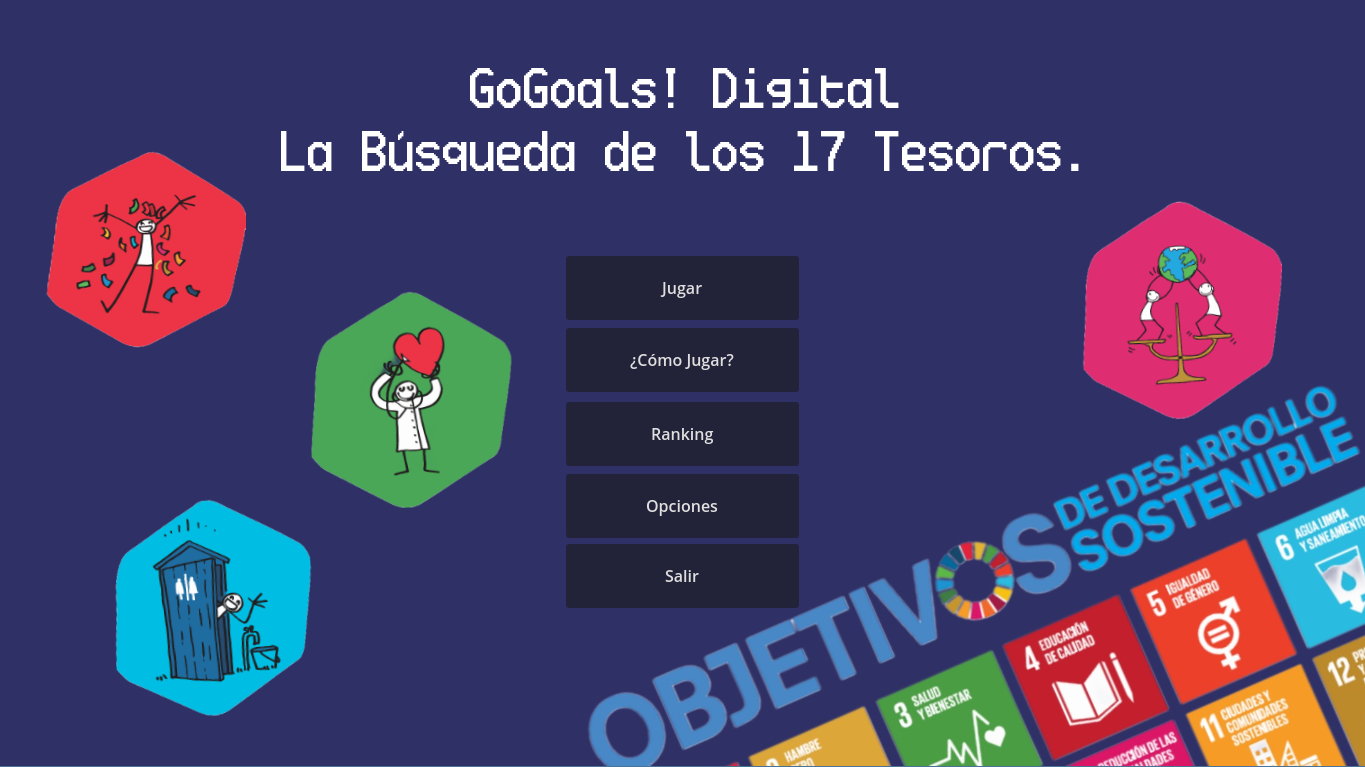
\includegraphics[width=0.85\textwidth]{Images/Menú Principal}
  \caption{Vista general del videojuego educativo \textit{Go Goals! Digital} (elaboración propia).\label{fig:propuesta_solucion}}
\end{figure}

Dentro del ecosistema de recursos educativos digitales sobre desarrollo sostenible, \textit{Go Goals! Digital} ocupa un nicho específico: es el único videojuego desarrollado en Cuba que adapta fielmente la mecánica del juego de mesa oficial de las Naciones Unidas a un entorno digital interactivo. A diferencia de otras iniciativas educativas basadas en vídeos o materiales estáticos, este videojuego integra la competencia entre varios jugadores, el azar controlado y la evaluación del conocimiento en una sola experiencia lúdica. La plataforma Godot Engine, elegida por su licencia libre MIT y su capacidad de exportación multiplataforma, garantiza la ejecución nativa en sistemas operativos de escritorio tales como Windows, Linux y macOS sin requerir configuraciones complejas, lo que resulta especialmente relevante en contextos educativos con recursos tecnológicos limitados.

El diseño del videojuego respeta los colores, íconos y denominaciones oficiales de cada ODS, lo que refuerza la identificación visual del contenido educativo y facilita su uso como complemento de programas curriculares relacionados con la sostenibilidad.

%---------------------------------------------------------------------------
\section{Planificación}
\label{sec:planificacion}

El presente epígrafe se enfoca en la organización y gestión del proyecto siguiendo la metodología Extreme Programming (XP). La planificación en XP se centra en la flexibilidad y la colaboración continua con el cliente, utilizando iteraciones cortas para adaptarse a cambios y priorizar funcionalidades \parencite{Beck2004}. Aquí se detallan los procesos clave que guían el desarrollo de \textit{Go Goals! Digital}, desde la obtención de requisitos hasta la definición de historias de usuario, la estimación de tiempo y el plan de iteraciones.

Como parte inicial de esta planificación, se realizaron sesiones de tormenta de ideas con el cliente para enfocar el proyecto en la arquitectura general, y posteriormente se llevaron a cabo reuniones que resultaron en la definición de los requisitos funcionales, no funcionales e historias de usuario.

\subsection{Requisitos funcionales}
\label{subsec:req_funcionales}

Los requisitos funcionales constituyen el conjunto de capacidades, comportamientos y procesos que un sistema debe implementar para satisfacer las necesidades de sus usuarios. Definen de manera precisa y verificable qué debe hacer el sistema: las entradas que procesa, las transformaciones que aplica y las salidas que produce \parencite{Sommerville2021, Pressman2019}. Para \textit{Go Goals! Digital}, los requisitos se obtuvieron mediante sesiones de trabajo con el cliente y el análisis de las mecánicas del juego de mesa original, priorizando las funcionalidades esenciales para la experiencia educativa.

\begin{longtable}{|c|p{0.3\textwidth}|p{0.37\textwidth}|c|c|}
\caption{Requisitos funcionales del videojuego Go Goals! Digital (elaboración propia).\label{tab:req_funcionales}} \\
\hline
\textbf{ID} & \textbf{Nombre} & \textbf{Descripción} & \textbf{Prioridad} & \textbf{Complejidad} \\
\hline
\endfirsthead
\multicolumn{5}{c}
{{ \tablename\ \thetable{} -- Continuación de la página anterior}} \\
\hline
\textbf{ID} & \textbf{Nombre} & \textbf{Descripción} & \textbf{Prioridad} & \textbf{Complejidad} \\
\hline
\endhead
\hline
RF-01 & Mostrar menú principal & El sistema debe contar con un menú principal con opciones de iniciar partida, ver instrucciones y salir. & Alta & Baja \\
\hline
RF-02 & Mostrar pantalla de instrucciones & El sistema debe mostrar las reglas del juego de manera clara y accesible. & Media & Baja \\
\hline
RF-03 & Iniciar partida & El sistema debe permitir al usuario iniciar una nueva partida configurando el número de jugadores hasta 4. & Alta & Baja \\
\hline
RF-04 & Visualizar tablero & El sistema debe mostrar el tablero hexagonal completo con las 63 casillas correctamente identificadas. & Alta & Media \\
\hline
RF-05 & Lanzar dado & El sistema debe simular el lanzamiento de un dado de 6 caras con resultado pseudoaleatorio. & Alta & Baja \\
\hline
RF-06 & Mover ficha & El sistema debe mover la ficha del jugador activo la cantidad de casillas indicada por el dado con animación. & Alta & Media \\
\hline
RF-07 & Aplicar efecto de escalera & El sistema debe detectar casillas de escalera y aplicar el avance correspondiente con animación. & Alta & Media \\
\hline
RF-08 & Aplicar efecto de serpiente & El sistema debe detectar casillas de serpiente y aplicar el retroceso correspondiente con animación. & Alta & Media \\
\hline
RF-09 & Mostrar pregunta ODS & El sistema debe mostrar una pregunta aleatoria del banco cuando una ficha cae en casilla temática. & Alta & Alta \\
\hline
RF-10 & Evaluar respuesta & El sistema debe evaluar la respuesta del jugador, mostrar retroalimentación y aplicar el efecto correspondiente. & Alta & Media \\
\hline
RF-11 & Gestionar turnos & El sistema debe gestionar el turno de cada jugador de forma automática y mostrar el jugador activo. & Alta & Media \\
\hline
RF-12 & Determinar condición de victoria & El sistema debe detectar cuando un jugador llega a la casilla 63 y mostrar la pantalla de victoria. & Alta & Baja \\
\hline
RF-13 & Mostrar estadísticas de partida & El sistema debe registrar y mostrar las respuestas correctas e incorrectas por jugador y por ODS. & Media & Alta \\
\hline
RF-14 & Configurar audio & El sistema debe permitir activar o desactivar música y efectos de sonido. & Baja & Baja \\
\hline
RF-15 & Pausar partida & El sistema debe permitir pausar la partida en cualquier momento y reanudarla desde el mismo estado. & Media & Baja \\
\hline
RF-16 & Reiniciar partida & El sistema debe permitir reiniciar la partida actual desde el inicio sin volver al menú principal. & Media & Baja \\
\hline
RF-17 & Habilitar cámara de seguimiento & El sistema debe incluir una cámara dinámica que enfoque automáticamente al jugador activo durante su turno. & Baja & Media \\
\hline
RF-18 & Habilitar modo de práctica & El sistema debe permitir al usuario jugar en solitario para recorrer el tablero, practicar y familiarizarse con el juego. & Media & Baja \\
\hline
\hline
\end{longtable}

\subsection{Requisitos no funcionales}
\label{subsec:req_no_funcionales}

Los requisitos no funcionales son aquellas especificaciones que describen cómo debe ser un sistema en términos de atributos de calidad, como rendimiento, seguridad, usabilidad y escalabilidad, en lugar de simplemente describir sus funciones. Estos requisitos se centran en aspectos como la eficiencia, confiabilidad y facilidad de mantenimiento del sistema, que son fundamentales para garantizar su éxito y aceptación por parte de los usuarios. Al considerar los requisitos no funcionales desde las etapas iniciales del desarrollo de software, se puede diseñar un sistema que cumpla con las expectativas de los usuarios en términos de calidad y experiencia de uso \parencite{Pressman2019}.

\textbf{Requisitos no funcionales de Usabilidad}

RNF-01: El sistema debe ser intuitivo y de fácil comprensión para usuarios de todas las edades.

RNF-02: Todos los textos de la interfaz deben renderizarse con una tipografía de tamaño igual o superior a 16pt para garantizar legibilidad.

RNF-03: Los botones interactivos principales deben poseer un área de colisión amplia y holgada para facilitar la interacción en pantallas táctiles y el acceso motriz.

RNF-04: La paleta de colores debe mantener un contraste alto entre el texto y el fondo, respetando los colores e íconos oficiales de los 17 ODS de las Naciones Unidas.

RNF-05: Al presentarse una funcionalidad nueva en la partida, el sistema debe mostrar una indicación o tutorial contextual breve.

\textbf{Requisitos no funcionales de Rendimiento}

RNF-06: El sistema debe responder a acciones del usuario, tales como lanzar el dado o seleccionar una respuesta, en menos de 0{,}5 segundos en hardware de gama media.

RNF-07: El ejecutable para Windows no debe superar los 150~MB para facilitar su distribución en contextos con ancho de banda limitado.

\textbf{Requisitos no funcionales de Software}

RNF-08: El videojuego debe ser compatible con Windows 10+, Linux (Ubuntu 20.04+) y macOS 11+.

RNF-09: La versión de escritorio debe funcionar completamente sin conexión a internet (disponibilidad offline).

RNF-10: El código GDScript debe mantener comentarios de documentación internos en todas las clases para garantizar la mantenibilidad.

\textbf{Requisitos no funcionales de Hardware}

RNF-11: El dispositivo debe poseer un procesador de doble núcleo a 1{,}5~GHz o superior.

RNF-12: El sistema debe contar con al menos 512~MB de memoria RAM disponible para la ejecución del videojuego.

RNF-13: Se debe disponer de al menos 300~MB de espacio libre en la unidad de almacenamiento para la instalación del ejecutable y sus archivos de datos.

\subsection{Historias de usuario}
\label{subsec:historias_usuario}

Las historias de usuario son una técnica fundamental en metodologías ágiles como Extreme Programming (XP), utilizadas para capturar requisitos desde la perspectiva del usuario final. Según \citeauthor{Cohn2005} \parencite{Cohn2005}, una historia de usuario es ``una descripción breve y simple de una funcionalidad deseada, expresada en lenguaje cotidiano y centrada en el valor que aporta al usuario''. A diferencia de los documentos de requisitos tradicionales, las historias de usuario son más flexibles, pero siguen el formato estandarizado:

\begin{center}
\textit{``Como [rol], quiero [acción], para [beneficio]''}
\end{center}

A continuación se presenta, a modo representativo, la historia de usuario más destacada del videojuego por su relevancia en la asimilación del contenido (Tabla \ref{tab:hu9}). El conjunto completo de dieciocho historias de usuario que componen el \textit{Product Backlog} se encuentra listado en el Anexo \ref{anx:historias_usuario}.

\begin{table}[H]
\centering
\caption{Historia de usuario 9: Mostrar pregunta ODS (elaboración propia).\label{tab:hu9}}
\renewcommand{\arraystretch}{1.5}
\begin{tabular}{|p{0.45\textwidth}|p{0.45\textwidth}|}
\hline
\multicolumn{2}{|l|}{\textbf{Historia de Usuario}} \\
\hline
\textbf{Número:} 9 & \textbf{Nombre:} Mostrar pregunta ODS \\
\hline
\textbf{Prioridad:} Alta & \textbf{Riesgo:} Alto \\
\hline
\textbf{Puntos de estimación:} 5.0 & \textbf{Iteración asignada:} 3 \\
\hline
\multicolumn{2}{|p{0.945\textwidth}|}{\textbf{Descripción:} Como jugador quiero responder preguntas cuando caiga en una casilla temática de ODS para aprender interactivamente sobre la sostenibilidad.} \\
\hline
\multicolumn{2}{|p{0.945\textwidth}|}{\textbf{Observaciones:}
\vspace{-0.5em}
\begin{itemize}
    \setlength\itemsep{0em}
    \item El juego debe pausar el turno al caer en casilla temática.
    \item Se debe mostrar un panel modal con el ícono del ODS, el texto de la pregunta y las opciones de respuesta.
    \item Se selecciona una pregunta aleatoria sin repetir dentro de la sesión.
\end{itemize}
\vspace{-1em}
} \\
\hline
\end{tabular}
\end{table}

\subsection{Estimación de tiempo de desarrollo}
\label{subsec:estimacion}

Los puntos de estimación en el desarrollo ágil se utilizan para medir el esfuerzo relativo requerido para completar una historia de usuario, en lugar de estimar el tiempo exacto. Esto sirve para evaluar su complejidad, comparar historias de usuario y planificar las iteraciones \parencite{Cohn2005}.

\begin{longtable}{|c|p{0.45\textwidth}|c|}
\caption{Puntos de estimación por historia de usuario (elaboración propia).\label{tab:estimacion}} \\
\hline
\textbf{No. HU} & \textbf{Nombre} & \textbf{Puntos (días)} \\
\hline
\endfirsthead
\multicolumn{3}{c}%
{{\tablename\ \thetable{} -- Continuación de la página anterior}} \\
\hline
\textbf{No. HU} & \textbf{Nombre} & \textbf{Puntos (días)} \\
\hline
\endhead
\hline
\endfoot
\hline
\endlastfoot
1. & Mostrar menú principal & 1.0 \\
\hline
2. & Mostrar pantalla de instrucciones & 1.0 \\
\hline
3. & Iniciar partida & 2.0 \\
\hline
4. & Visualizar tablero & 5.0 \\
\hline
5. & Lanzar dado & 1.5 \\
\hline
6. & Mover ficha & 4.0 \\
\hline
7. & Aplicar efecto de escalera & 1.5 \\
\hline
8. & Aplicar efecto de serpiente & 1.5 \\
\hline
9. & Mostrar pregunta ODS & 5.0 \\
\hline
10. & Evaluar respuesta & 3.0 \\
\hline
11. & Gestionar turnos & 2.0 \\
\hline
12. & Determinar condición de victoria & 1.5 \\
\hline
13. & Mostrar estadísticas de partida & 4.0 \\
\hline
14. & Configurar audio & 2.5 \\
\hline
15. & Pausar partida & 1.0 \\
\hline
16. & Reiniciar partida & 1.0 \\
\hline
17. & Habilitar cámara de seguimiento & 2.0 \\
\hline
18. & Habilitar modo de práctica & 5.0 \\
\hline
\multicolumn{2}{|r|}{\textbf{Total}} & \textbf{44.5} \\
\hline
\end{longtable}

\subsection{Plan de iteraciones}
\label{subsec:plan_iteraciones}

El plan de iteraciones es una herramienta esencial para organizar y coordinar el trabajo del equipo de desarrollo siguiendo la metodología Extreme Programming. Cada iteración se planifica con una duración de una a tres semanas y comienza con una reunión de planificación en la que el cliente presenta las historias de usuario priorizadas, y el equipo de desarrollo estima y se compromete a completar las tareas necesarias \parencite{Cohn2005}. Al finalizar cada iteración, se entrega un incremento funcional del software que puede ser evaluado por el cliente, cerrando el ciclo de retroalimentación y permitiendo ajustar las prioridades para la iteración siguiente \parencite{Beck2004}.

Para \textit{Go Goals! Digital}, el desarrollo se organizó en cinco iteraciones que siguen una progresión lógica: las dos primeras sientan las bases del proyecto; la tercera integra el núcleo pedagógico; la cuarta incorpora funcionalidades de cierre y configuración; y la quinta agrega características complementarias que mejoran la experiencia de usuario. Esta estructura permite validar tempranamente las funcionalidades de mayor riesgo técnico, como la visualización del tablero hexagonal y el motor de preguntas, antes de proceder con los componentes de menor complejidad.

\begin{longtable}{|c|c|p{0.45\textwidth}|c|}
\caption{Plan de iteraciones de desarrollo (elaboración propia).\label{tab:plan_iteraciones}} \\
\hline
\textbf{Iteración} & \textbf{No. HU} & \textbf{Historia de Usuario} & \textbf{Duración (días)} \\
\hline
\endfirsthead
\multicolumn{4}{c}%
{{\tablename\ \thetable{} -- Continuación de la página anterior}} \\
\hline
\textbf{Iteración} & \textbf{No. HU} & \textbf{Historia de Usuario} & \textbf{Duración (días)} \\
\hline
\endhead
\hline
\endfoot
\hline
\endlastfoot
\multirow{4}{*}{1} & 1 & Mostrar menú principal & \multirow{4}{*}{9.0} \\
\cline{2-3}
 & 2 & Mostrar pantalla de instrucciones & \\
\cline{2-3}
 & 3 & Iniciar partida & \\
\cline{2-3}
 & 4 & Visualizar tablero & \\
\hline
\multirow{4}{*}{2} & 5 & Lanzar dado & \multirow{4}{*}{8.5} \\
\cline{2-3}
 & 6 & Mover ficha & \\
\cline{2-3}
 & 7 & Aplicar efecto de escalera & \\
\cline{2-3}
 & 8 & Aplicar efecto de serpiente & \\
\hline
\multirow{3}{*}{3} & 9 & Mostrar pregunta ODS & \multirow{3}{*}{10.0} \\
\cline{2-3}
 & 10 & Evaluar respuesta & \\
\cline{2-3}
 & 11 & Gestionar turnos & \\
\hline
\multirow{5}{*}{4} & 12 & Determinar condición de victoria & \multirow{5}{*}{10.0} \\
\cline{2-3}
 & 13 & Mostrar estadísticas de partida & \\
\cline{2-3}
 & 14 & Configurar audio & \\
\cline{2-3}
 & 15 & Pausar partida & \\
\cline{2-3}
 & 16 & Reiniciar partida & \\
\hline
\multirow{2}{*}{5} & 17 & Habilitar cámara de seguimiento & \multirow{2}{*}{7.0} \\
\cline{2-3}
 & 18 & Habilitar modo de práctica & \\
\hline
\multicolumn{3}{|r|}{\textbf{Total}} & \textbf{44.5} \\
\hline
\end{longtable}

%---------------------------------------------------------------------------
\section{Diseño}
\label{sec:diseno}

El presente epígrafe constituye la transición esencial entre la planificación teórica y la implementación práctica, donde se materializan los requisitos en soluciones técnicas concretas. Este apartado se centra en tres pilares fundamentales: la arquitectura del sistema, que detalla cómo la estructura basada en nodos y el SceneTree de Godot permiten organizar los componentes clave del videojuego; los prototipos de interfaces gráficas de usuario; y las tarjetas CRC que definen la interacción entre las clases del sistema.

\subsection{Arquitectura Jerárquica Basada en Nodos}
\label{subsec:arquitectura}

Godot Engine utiliza una arquitectura jerárquica basada en nodos, la cual es identificada como el árbol de escenas. En esta arquitectura, los \textbf{nodos} son los bloques de construcción fundamentales: cada elemento del videojuego, desde una ficha de jugador hasta un efecto de sonido, es un nodo que hereda de la clase base \texttt{Node}. Los nodos se organizan en \textbf{escenas}, que son composiciones reutilizables de nodos agrupados jerárquicamente; una escena puede representar desde un botón hasta una pantalla completa del juego. El \textbf{SceneTree} es la estructura global que gestiona todas las escenas y nodos en tiempo de ejecución, funcionando como un árbol de procesamiento que organiza el orden de ejecución de métodos, la jerarquía de transformaciones y la gestión de señales que comunican a los nodos entre sí \parencite{GodotDocs2026}.

El uso del SceneTree aporta ventajas significativas para \textit{Go Goals! Digital}. En primer lugar, aumenta la modularidad al permitir tener una escena para cada funcionalidad específica, como podría ser una ficha de jugador, que puede instanciarse dentro de otra escena más grande como el tablero. De esta manera, el tablero puede contener varias fichas, cada una con sus propiedades individuales (color, posición, nombre del jugador). Al momento de necesitar cambiarlas todas, se pueden realizar modificaciones en la escena de la ficha, reflejándose automáticamente en todas las instancias. Otra ventaja es el rendimiento, que mejora debido a que evita actualizaciones innecesarias y permite operaciones masivas como llamadas de métodos en grupos de nodos. Su diseño trae un enfoque de composición sobre herencia para no depender de jerarquías rígidas de clases y posee funcionalidades para realizar cambios de escenas de forma fluida.

La comunicación entre estos elementos se simplifica gracias al sistema de señales integrado, permitiendo que eventos como el lanzamiento del dado, el movimiento de fichas o la presentación de preguntas se coordinen eficientemente sin acoplamiento rígido entre componentes. Además, el SceneTree optimiza automáticamente el rendimiento al gestionar el orden de procesamiento y renderizado, algo relevante en un juego de tablero donde múltiples fichas, animaciones y elementos de interfaz pueden interactuar simultáneamente en pantalla. La capacidad de pausar o manipular selectivamente ramas enteras del árbol de escenas es particularmente útil para implementar mecánicas como el menú de pausa o la transición entre el tablero y el panel de preguntas educativas.

\begin{figure}[!htbp]
  \centering
  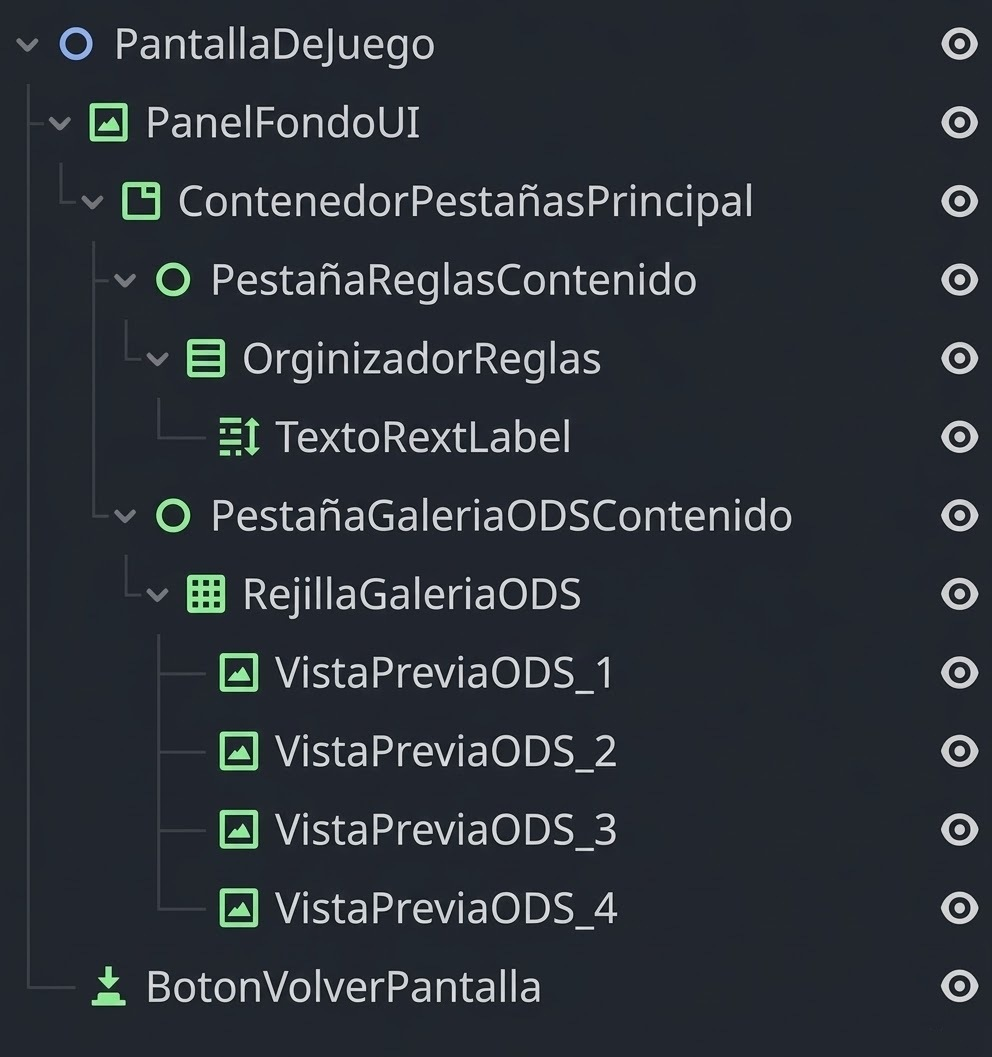
\includegraphics[width=0.55\textwidth]{Images/SceeneTree}
  \caption{Ejemplo de jerarquía de nodos en el SceneTree de Godot: pantalla de instrucciones del videojuego \textit{Go Goals! Digital} (elaboración propia).\label{fig:scene_tree}}
\end{figure}

El videojuego \textit{Go Goals! Digital} emplea esta Arquitectura Jerárquica Basada en Nodos, apoyada por servicios globales y coordinada centralmente. Esta elección arquitectural no es arbitraria: frente a alternativas como un patrón \textit{Model-View-Controller} clásico o una separación por capas estricta, la composición de nodos de Godot resulta superior para este proyecto por razones concretas de extensibilidad y mantenibilidad. Un MVC rígido tendería a concentrar en el controlador una cantidad creciente de lógica de presentación a medida que se incorporen nuevas mecánicas, como nuevos tipos de casillas o modos de juego, generando un acoplamiento progresivo entre la vista y el controlador. La composición orientada a nodos, en cambio, permite agregar una nueva funcionalidad como un nodo hijo con su propio script, sin tocar el controlador principal. Esto favorece directamente la extensibilidad y reduce el riesgo de regresiones al modificar el sistema. Como buena práctica de diseño, se estructuró el proyecto en cuatro pilares fundamentales de responsabilidad:

\begin{itemize}
    \item \textbf{Arquitectura Orientada a Escenas}: La navegación principal y los límites de las interfaces dependen del sistema nativo de escenas de Godot. Entornos como el menú principal, la pantalla de juego interactiva y el menú de fin de partida funcionan como fronteras naturales de presentación. Dentro del juego, el nivel principal actúa como controlador de composición local, ensamblando las dependencias y conectando la interfaz de usuario con la lógica sin mezclar directamente sus responsabilidades.
    
    \item \textbf{Servicios Globales y Autoloads}: Godot facilita el patrón Singleton a través de nodos que se registran globalmente, permitiendo el acceso a funcionalidades transversales desde cualquier escena. El proyecto emplea la clase \texttt{GameData} para mantener la configuración de la partida y cargar el banco de preguntas; \texttt{AudioManager} para centralizar la reproducción de música y efectos de sonido; y \texttt{RecordsManager} para gestionar la persistencia local de las puntuaciones de forma estructurada e independiente.
    
    \item \textbf{Coordinación Central y Comunicación por Eventos}: El flujo del juego es orquestado por el coordinador central \texttt{GameManager}. Este componente concentra los casos de uso principales, como el control de turnos, el movimiento, las preguntas y la victoria. La comunicación hacia la interfaz gráfica no se realiza mediante referencias directas entre escenas invocando \texttt{get\_node()}, ya que ello generaría un acoplamiento temporal rígido: si la escena destino aún no está cargada, el sistema colapsaría. En su lugar, se emplea un bus de señales globales implementado en \texttt{GameEvents}, de modo que componentes como el panel de preguntas reaccionan de manera completamente independiente a los eventos emitidos, sin conocer ni depender del código del coordinador. Esto desacopla emisor y receptor, facilita la escalabilidad y permite añadir nuevos suscriptores sin modificar el núcleo lógico.
    
    \item \textbf{Modelo de Estado Separado y Entidades Ligeras}: El estado mutable de la partida, que incluye la fase del juego, el turno actual y la cantidad de tiradas, se aísla en un modelo de estado explícito programado en \texttt{GameState}, lo cual facilita administrar pausas o finalizaciones. Adicionalmente, el dominio se representa a través de entidades interactivas ligeras que encapsulan su comportamiento particular, pero que delegan el control de flujo global al coordinador de la partida.
\end{itemize}

\subsubsection{Estructura de directorios del proyecto}
\label{subsubsec:capas}

La organización del código fuente sigue una estructura jerárquica por responsabilidad funcional, coherente con los principios de alta cohesión y bajo acoplamiento \parencite{Pressman2019}:

\begin{itemize}
    \item \textbf{autoloads/}: contiene los Singletons globales del proyecto (\texttt{GameData}, \texttt{AudioManager}, \texttt{RecordsManager}).
    \item \textbf{scripts/Core/}: contiene los archivos de infraestructura del ciclo de vida del juego, como el bus de eventos en \texttt{Events.gd} y la m\'aquina de estados en \texttt{GameState.gd}.
    \item \textbf{scripts/Data/}: contiene el archivo de configuración estática del tablero en \texttt{BoardConfig.gd}, donde se definen todas las casillas de escaleras, toboganes y preguntas con sus posiciones de origen y destino.
    \item \textbf{scripts/Entities/}: contiene los objetos del dominio del juego, específicamente \texttt{Board.gd}, \texttt{Player.gd} y \texttt{Tile.gd}, que encapsulan propiedades pero no decisiones.
    \item \textbf{scripts/Managers/}: contiene el \texttt{GameManager.gd}, controlador central que orquesta el ciclo de la partida.
    \item \textbf{scripts/UI/}: contiene los scripts de la capa de presentación, incluyendo los paneles del tablero, el panel de preguntas, el menú de pausa y la pantalla de estadísticas.
\end{itemize}

\subsection{Prototipos de interfaces gráficas}
\label{subsec:prototipos}

En el presente epígrafe se presentan las principales interfaces gráficas del videojuego en su forma de prototipo, describiendo cada uno de sus elementos y las funcionalidades asociadas. El diseño de las interfaces gráficas prioriza la accesibilidad, comprensibilidad y atractivo visual apto para todas las edades, manteniendo fidelidad a los colores e íconos oficiales de los diecisiete ODS.

\begin{figure}[H]
  \centering
  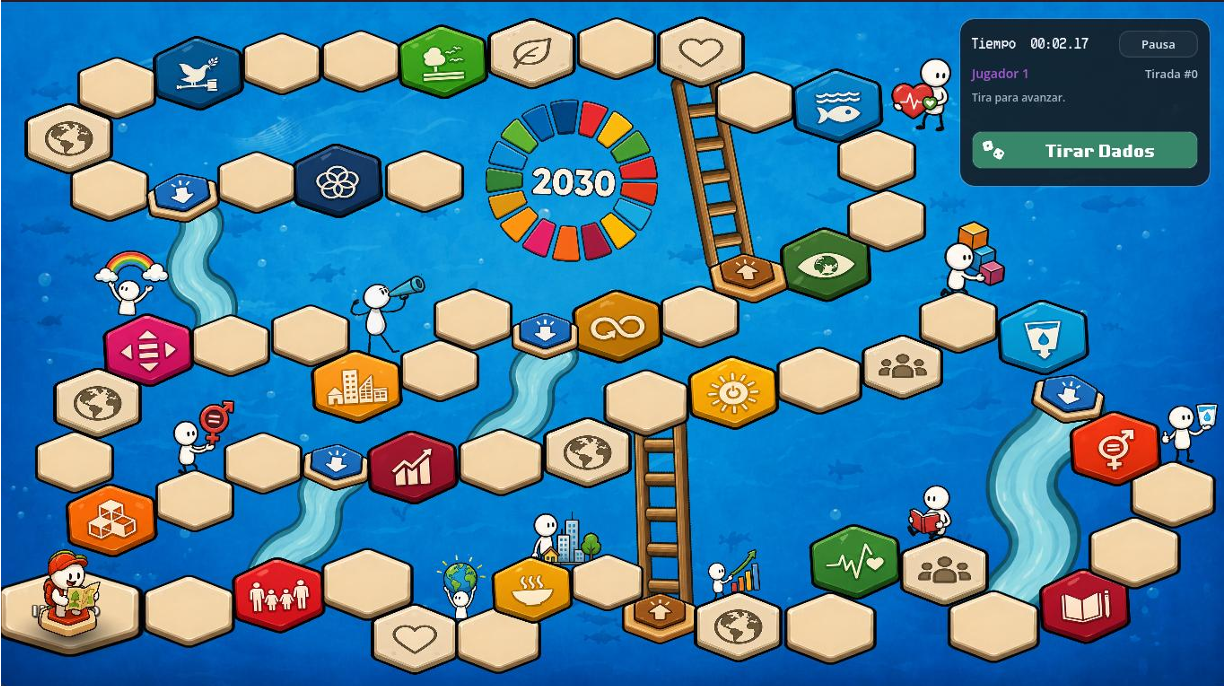
\includegraphics[width=0.7\textwidth]{Images/GoGoals Digital}
  \caption{Prototipo de la pantalla principal del tablero de juego (elaboración propia).\label{fig:prototipo_tablero}}
\end{figure}

\subsubsection{Panel de preguntas educativas}
\label{subsubsec:panel_preguntas}

El panel de preguntas constituye el componente central de la experiencia educativa del videojuego, ya que es el espacio donde se materializa la evaluación del conocimiento sobre los ODS. Este elemento funciona como una interfaz modal que se superpone al tablero durante las casillas temáticas, pausando temporalmente el flujo del juego para concentrar la atención del jugador en el contenido pedagógico. Su diseño responde a la necesidad de crear un momento de reflexión y aprendizaje dentro de la dinámica lúdica, equilibrando la competencia con la adquisición de conocimientos.

Tras la selección de una respuesta, el panel transita a un estado de retroalimentación que muestra un indicador visual claro (verde para correcto, rojo para incorrecto) acompañado de una breve explicación pedagógica que refuerza el aprendizaje. Esta retroalimentación permanece visible durante aproximadamente 5 segundos antes de cerrar el panel y continuar el turno, permitiendo que el jugador asimile la información sin interrumpir excesivamente el ritmo del juego.

\begin{figure}[H]
  \centering
  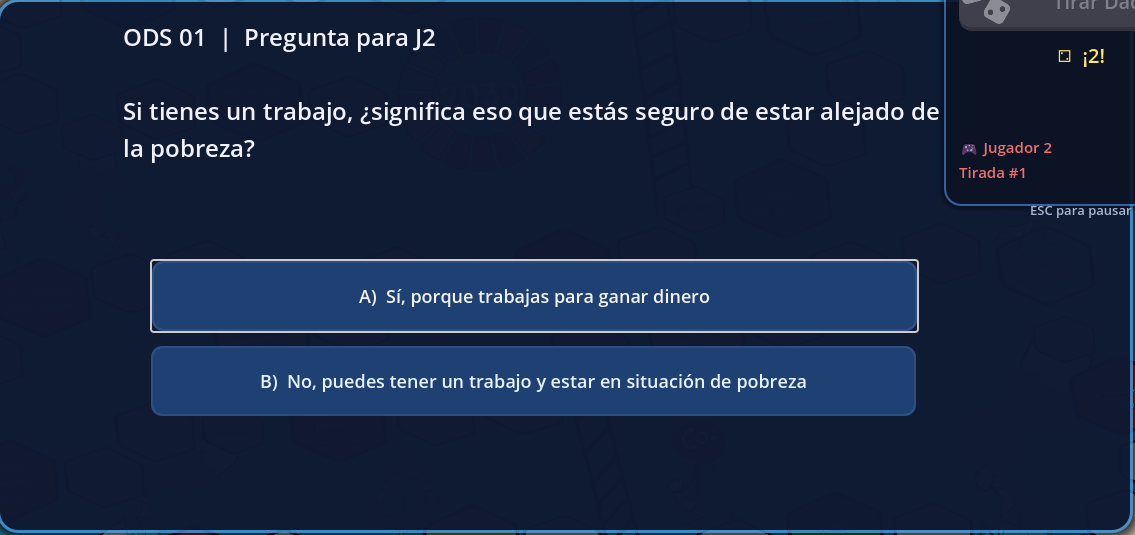
\includegraphics[width=0.75\textwidth]{Images/Panel Preguntas}
  \caption{Prototipo del panel de preguntas educativas por ODS (elaboración propia).\label{fig:prototipo_preguntas}}
\end{figure}

\subsubsection{Pantalla de estadísticas}
\label{subsubsec:pantalla_estadisticas}

La pantalla de estadísticas se presenta al finalizar la partida y constituye uno de los elementos más importantes desde el punto de vista pedagógico del videojuego. Esta interfaz muestra una tabla de clasificación ordenada que permite visualizar el desempeño comparativo de todos los jugadores participantes. La tabla presenta información estructurada en columnas que incluyen la posición final de cada jugador, el número de turnos que necesitó para completar el recorrido, el tiempo total invertido en la partida y el nombre del participante.

El criterio principal de ordenamiento es el número de turnos, considerando que un menor número de turnos indica un mejor desempeño en el conocimiento de los ODS, ya que implica menos retrocesos por respuestas incorrectas. En caso de empate en el número de turnos, el sistema utiliza el tiempo como criterio de desempate, favoreciendo al jugador que completó el recorrido en menor tiempo. Esta mecánica de clasificación incentiva tanto la precisión en las respuestas como la agilidad en la toma de decisiones.

\begin{figure}[H]
  \centering
  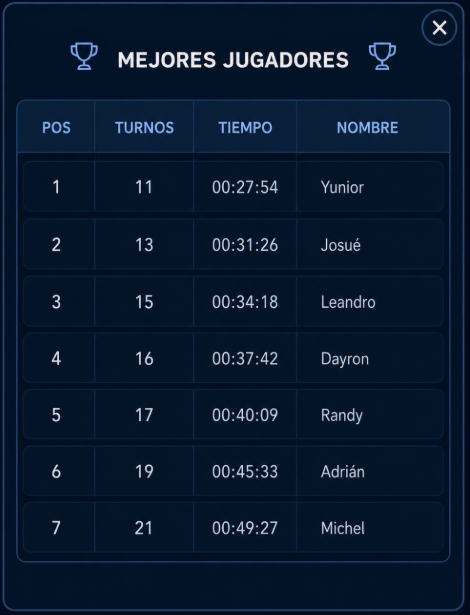
\includegraphics[width=0.35\textwidth]{Images/Ranking}
  \caption{Prototipo de la pantalla de estadísticas y clasificación final (elaboración propia).\label{fig:prototipo_estadisticas}}
\end{figure}

\subsection{Tarjetas CRC}
\label{subsec:tarjetas_crc}

Las tarjetas de clase, responsabilidad y colaboración constituyen una técnica fundamental en el diseño ágil, particularmente relevante en la metodología Extreme Programming. Son una herramienta efectiva para la conceptualización y diseño de sistemas orientados a objetos, que facilita la identificación de las clases, sus responsabilidades y las colaboraciones necesarias entre ellas \parencite{Sommerville2021}. A continuación se presenta, a modo ilustrativo, la tarjeta CRC del controlador principal del juego representado por la clase \texttt{GameManager} en la Tabla \ref{tab:crc_gamemanager}. El conjunto completo de las diez tarjetas CRC con el detalle arquitectónico restante se encuentra listado en el Anexo \ref{anx:tarjetas_crc}.

\begin{table}[H]
\centering
\caption{Tarjeta CRC GameManager (Controlador) (elaboración propia).\label{tab:crc_gamemanager}}
\begin{tabular}{|p{0.25\textwidth}|p{0.64\textwidth}|}
\hline
\multicolumn{2}{|c|}{\textbf{Tarjeta CRC}} \\
\hline
\textbf{Clase:} & GameManager \\
\hline
\textbf{Responsabilidades} & - orquestar el ciclo completo de la partida (inicio, turno, resolución de casilla, fin) \\
& - calcular rutas de movimiento e invocar animaciones \\
& - verificar condiciones de victoria \\
\hline
\textbf{Clases relacionadas} & GameState \\
& GameEvents \\
& BoardConfig \\
& AudioManager \\
\hline
\end{tabular}
\end{table}

La separación de responsabilidades reflejada en la tarjeta CRC de \texttt{GameManager} responde a una decisión concreta de diseño: centralizar el flujo evita que la lógica del turno quede dispersa en múltiples nodos de la interfaz, lo que generaría un acoplamiento implícito difícil de rastrear. Al delegar en \texttt{GameEvents} la notificación de cambios a la UI y en \texttt{GameState} la gestión del estado, el \texttt{GameManager} se mantiene cohesivo y reemplazable: cualquier componente de la interfaz que deba reaccionar a un evento de juego lo hace suscribiéndose a una se\~nal global, sin crear una dependencia directa con el controlador. Esta arquitectura elimina el acoplamiento temporal entre la lógica y la presentación, y simplifica las pruebas al poder invocar el controlador sin necesidad de instanciar la interfaz completa.



%---------------------------------------------------------------------------
\section{Implementación}
\label{sec:implementacion}

El presente epígrafe describe el proceso de implementación del videojuego educativo \textit{Go Goals! Digital}, abordando los estándares de codificación adoptados, los patrones de diseño aplicados y las tareas de ingeniería ejecutadas en cada iteración.

\subsection{Estándares de codificación}
\label{subsec:estandares}

Los estándares de codificación son un conjunto de convenciones y reglas que guían la forma en que se escribe el código fuente de un sistema, con el objetivo de mejorar su legibilidad, mantenibilidad y consistencia. Según \citeauthor{Sommerville2021} \parencite{Sommerville2021}, el cumplimiento de estándares de codificación es un factor clave para reducir la deuda técnica y facilitar la colaboración en equipos de desarrollo.

\subsubsection{Nomenclatura y estructura de archivos}
\label{subsubsec:nomenclatura}

Para el desarrollo en GDScript se aplicaron los siguientes estándares de nomenclatura, coherentes con las convenciones oficiales de la documentación de Godot \parencite{GodotDocs2026}. Estas convenciones facilitan la legibilidad del código y permiten que cualquier desarrollador familiarizado con Godot pueda comprender rápidamente la estructura del proyecto:

\begin{itemize}
    \item \textbf{Clases}: PascalCase, por ejemplo \texttt{GameManager} y \texttt{QuestionManager}.
    \item \textbf{Variables y funciones}: snake\_case, como \texttt{current\_player} y \texttt{roll\_dice()}.
    \item \textbf{Constantes}: SCREAMING\_SNAKE\_CASE, tales como \texttt{MAX\_PLAYERS} y \texttt{BOARD\_SIZE}.
    \item \textbf{Señales}: snake\_case prefijadas con el evento, por ejemplo \texttt{dice\_rolled} y \texttt{answer\_checked}.
    \item \textbf{Escenas}: PascalCase coincidiendo con el nombre de su script raíz, como \texttt{GameBoard.tscn}.
\end{itemize}

La arquitectura de directorios del proyecto obedece a una distribución basada en características funcionales, enfoque metodológico que agrupa componentes afines en espacios de trabajo claramente delimitados. En lugar de consolidar archivos únicamente por su formato u origen, el árbol segmenta los recursos en tres ramas principales. Primeramente, el directorio \texttt{assets} se encarga de aislar la multimedia estática transversal, albergando módulos de audio, fuentes tipográficas y elementos gráficos del tablero tales como los tokens o los tipos de hexágonos. Seguidamente, el bloque de \texttt{escenas} aloja las vistas empaquetadas instanciables, ilustradas por pantallas clave estilo \texttt{GameBoard} o \texttt{QuizView}. Por último, el núcleo lógico se aísla en la rama \texttt{scripts}, subdividida internamente en \texttt{clases} de entidad y componentes \texttt{singletons} de acceso global. Esta estricta separación semántica mitiga los tiempos de búsqueda, protege frente a la ruptura conflictiva de referencias internas propias del motor, y facilita que la escalabilidad a largo plazo del código base se sostenga de forma limpia y disciplinada:

\begin{figure}[H]
  \centering
  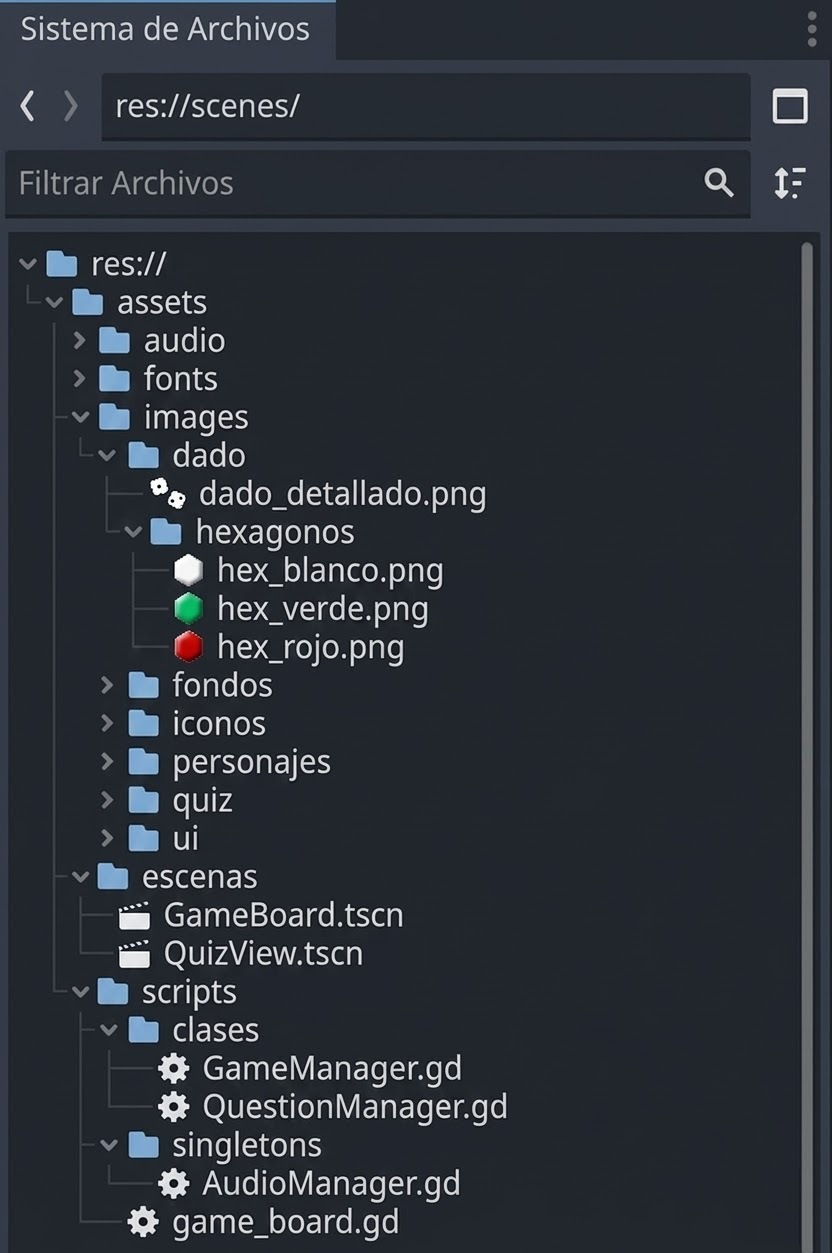
\includegraphics[width=0.35\textwidth]{Images/Jerarquia}
  \caption{Estructura de archivos del proyecto \textit{Go Goals! Digital} (elaboración propia).\label{fig:estructura_archivos}}
\end{figure}

\subsubsection{Documentación del código}
\label{subsubsec:documentacion_codigo}

Cada clase implementada en GDScript incluye comentarios de documentación al inicio del archivo describiendo su propósito, y comentarios de bloque en funciones de lógica compleja. Esta práctica facilita el mantenimiento futuro del código y permite la incorporación de nuevos desarrolladores al proyecto \parencite{GodotDocs2026}.

\subsection{Patrones de diseño utilizados}
\label{subsec:patrones}

Los patrones de diseño son soluciones reutilizables a problemas recurrentes en el desarrollo de software. Estos patrones proporcionan una manera estandarizada de abordar tareas de diseño recurrentes, mejorando la eficiencia y la coherencia del código. Al emplear patrones de diseño, los desarrolladores pueden beneficiarse de soluciones probadas que facilitan la comunicación, el mantenimiento y la extensibilidad del software \parencite{Pressman2019}. \textit{Go Goals! Digital} aplica los siguientes patrones de diseño, reflejados directamente en la estructura del código fuente.

\subsubsection{Patrones GRASP}
\label{subsubsec:patrones_grasp}

Son un conjunto de principios para asignar responsabilidades y funciones en el diseño de software orientado a objetos. Estos patrones ayudan a los desarrolladores a tomar decisiones coherentes sobre dónde ubicar la funcionalidad dentro del sistema. Al aplicar estos principios, se puede lograr un diseño de software más modular, flexible y fácil de mantener \parencite{Pressman2019}.

\textbf{Controlador de Fachada}

Tiene como objetivo asignar la responsabilidad de manejar las solicitudes del usuario a un componente específico, llamado controlador. En el proyecto, el script \texttt{GameManager.gd} centraliza la orquestación del ciclo de juego, delegando las tareas a otros objetos según sea necesario y coordinando el flujo general de la partida.

\textbf{Experto en información}

Se centra en asignar responsabilidades a la clase que posee la mayor cantidad de información necesaria para cumplir con dicha responsabilidad. Los modelos del proyecto, específicamente \texttt{Board.gd}, \texttt{Player.gd} y \texttt{Tile.gd}, encapsulan sus propias propiedades y aplican este principio, asegurando que cada entidad gestione únicamente sus propios datos.

\textbf{Bajo acoplamiento}

Este principio busca minimizar las dependencias entre las clases, lo que reduce el impacto de los cambios. Es notable que la configuración estática del tablero se aísla en \texttt{BoardConfig.gd}, separando los datos (escaleras, toboganes y casillas de quiz) de la lógica. Esta decisión de diseño garantiza que el sistema sea fácilmente extensible ante futuras modificaciones del tablero o las reglas del juego sin alterar el controlador principal.

\subsubsection{Patrones GOF}
\label{subsubsec:patrones_gof}

Los patrones de diseño GOF (Gang of Four) actúan como directrices estructuradas y probadas que brindan a los desarrolladores un marco sólido para abordar desafíos específicos organizados en categorías como creacionales, estructurales y de comportamiento.

\textbf{Singleton}

Garantiza que una clase tenga una única instancia y proporciona un punto de acceso global a ella. Godot implementa este patrón de forma nativa mediante el mecanismo de Autoloads. Los Autoloads del proyecto son \texttt{GameData} (repositorio central), \texttt{AudioManager} (gestión de sonido global) y \texttt{RecordsManager} (persistencia de datos), permitiendo que cualquier nodo acceda a estos servicios sin dependencias cruzadas \parencite{GodotDocs2026}.

\textbf{Observer (Bus de Eventos)}

Define una dependencia de uno-a-muchos entre objetos. El archivo \texttt{GameEvents} implementa una variante de este patrón a nivel de bus de eventos global. En lugar de conectar directamente un emisor con sus suscriptores, define se\~nales globales como \texttt{dice\_rolled} y \texttt{quiz\_requested} que cualquier componente emite o escucha de forma independiente, eliminando el acoplamiento entre el controlador y los componentes de la interfaz gráfica de usuario.

\begin{figure}[H]
  \centering
  \makebox[\textwidth]{\includegraphics[width=1.1\textwidth]{Images/signals}}
  \caption{Patrón Observer implementado mediante señales globales en Godot (elaboración propia).\label{fig:senales_godot}}
\end{figure}

\textbf{State (Máquina de Estados)}

Permite a un objeto alterar su comportamiento cuando su estado interno cambia. La alternativa más simple habría sido gestionar el estado de la partida mediante variables booleanas independientes, como \texttt{is\_paused}, \texttt{is\_rolling} e \texttt{is\_answering}. Sin embargo, este enfoque introduce de inmediato un problema estructural: las combinaciones de banderas pueden coexistir en estados inválidos, por ejemplo permitiendo que \texttt{is\_rolling = true} e \texttt{is\_answering = true} ocurran simultáneamente, generando condiciones de carrera y sentencias \texttt{if/else} anidadas que se vuelven inmanejables a medida que crece el sistema. El patrón \textit{State}, implementado en \texttt{GameState.gd} mediante una enumeración explícita de fases que abarca \texttt{MENU}, \texttt{PLAYING}, \texttt{PAUSED} y \texttt{GAME\_OVER}, garantiza que el sistema se encuentre en un único estado válido en cada instante. Las transiciones son atómicas y verificables, lo que simplifica la depuración, facilita las operaciones de guardado y restauración de estado y hace que el comportamiento del sistema sea predecible ante cualquier secuencia de eventos.

\subsubsection{Manejo de datos y persistencia}
\label{subsubsec:manejo_datos}

La arquitectura del videojuego exige un manejo robusto de los datos, separando la configuración persistente del estado efímero de la partida. Para ello, el Singleton \texttt{GameData} actúa como repositorio en memoria, mientras que \texttt{RecordsManager} se encarga de serializar y almacenar localmente las estadísticas de los jugadores en el sistema de archivos del usuario. El contenido pedagógico, que incluye el banco de preguntas por cada ODS, se almacena externamente en formato JSON, permitiendo actualizar el cuestionario sin necesidad de recompilar el proyecto.

El sistema implementa manejo de excepciones en los puntos críticos de entrada de datos. Ante la ausencia o invalidez sintáctica del archivo \texttt{questions.json}, se interrumpe la ejecución y se despliega una alerta: \textit{«Questions file not found or invalid. Please verify that \texttt{questions.json} exists in the data directory.»} Esta detención es intencional: el núcleo pedagógico del videojuego depende del banco de preguntas, por lo que carece de sentido continuar sin él. La validación semántica de cada pregunta se delega al redactor del archivo JSON, no al motor de juego, dado que el banco está diseñado para ser editado por educadores sin intervención del compilador.

\subsection{Tareas de ingeniería}
\label{subsec:tareas_ingenieria}

Las tareas de ingeniería son los componentes técnicos específicos derivados de las historias de usuario. Representan el trabajo concreto que debe realizarse para implementar cada funcionalidad. A continuación se expone de manera representativa, en la Tabla \ref{tab:ti5}, la tarea de ingeniería responsable del manejo interactivo de los ODS, vinculada a las HU9 y HU10 explicadas anteriormente. El conjunto completo con las diez tareas de ingeniería organizadas por iteración se encuentra disponible en el Anexo \ref{anx:tareas_ingenieria}.

\begin{table}[H]
\centering
\caption{Tarea de ingeniería 5: Sistema de preguntas y evaluación de respuestas (elaboración propia).\label{tab:ti5}}
\begin{tabular}{|p{0.3\textwidth}|p{0.65\textwidth}|}
\hline
\textbf{Campo} & \textbf{Descripción} \\
\hline
Tarea \# & 5 \\
\hline
HU relacionada & HU \#9, HU \#10 \\
\hline
Nombre & Implementación del sistema de preguntas y retroalimentación \\
\hline
Tipo & Desarrollo \\
\hline
Puntos estimados & 8.0 días \\
\hline
Iteración & 3 \\
\hline
Programador & Ruslan Alexei Martinez Campos \\
\hline
Descripción & Se integra el motor de lectura JSON para cargar preguntas ODS y se programa el panel modal interactivo para evaluar y retroalimentar al jugador. \\
\hline
\end{tabular}
\end{table}



%---------------------------------------------------------------------------
\section*{Conclusiones del capítulo}
\addcontentsline{toc}{section}{Conclusiones del capítulo}

El diseño del sistema a partir de los requisitos funcionales y no funcionales, plasmados en 18 historias de usuario y organizados en 5 iteraciones ágiles, confirmó la pertinencia de la metodología Extreme Programming para proyectos de software educativo de pequeña escala, al garantizar entregas incrementales y adaptación continua a las prioridades del cliente.

La arquitectura jerárquica basada en nodos de Godot, coordinada mediante servicios globales y un bus de eventos desacoplado, resultó la elección más adecuada para el proyecto por favorecer la extensibilidad de mecánicas y la mantenibilidad del código, al tiempo que la aplicación de los patrones GRASP y GoF (Singleton, Observer y State) aportó soluciones técnicas probadas a los problemas de gestión de estado, comunicación entre componentes y persistencia de datos.

La implementación de las diez tareas de ingeniería, bajo los estándares de codificación GDScript y con contenido educativo externalizado en formato JSON con validación de integridad, produjo un videojuego educativo funcional, de bajo peso, multiplataforma y con mecanismos de robustez ante errores en los datos, cumpliendo así con el objetivo propuesto en la investigación.


  \chapter{Validación}
\label{chap:chapter3}

El presente capítulo aborda la validación del videojuego educativo \textit{Go Goals! Digital} mediante la aplicación sistemática de pruebas de software. La estructura del capítulo se organiza en dos secciones principales: la primera describe el diseño metodológico de la validación, especificando los tipos de pruebas empleados conforme a los estándares de la metodología Extreme Programming; la segunda presenta los resultados obtenidos tras la ejecución de dichas pruebas, evidenciando el cumplimiento de los requerimientos funcionales y no funcionales establecidos para el sistema.

%---------------------------------------------------------------------------
\section{Proceso de pruebas de software}
\label{sec:diseno_validacion}

Este epígrafe presenta los tipos de pruebas utilizados en el ciclo de desarrollo del videojuego \textit{Go Goals! Digital}, siguiendo la metodología XP.

Las pruebas de software evalúan y verifican la calidad y correcto funcionamiento de un sistema informático, asegurando que cumpla con los requerimientos técnicos y las expectativas del usuario final. Se clasifican en pruebas de caja blanca, que examinan la estructura interna del código, y pruebas de caja negra, que validan el comportamiento externo sin conocer la implementación. La combinación de pruebas manuales y automatizadas permite identificar errores de forma temprana, optimizar los tiempos de corrección y garantizar la estabilidad del software, lo que es fundamental en entornos de desarrollo ágil e iterativo \parencite{Pressman2019}.

\subsection{Tipos de pruebas}
\label{subsec:tipos_pruebas}

En \textit{Go Goals! Digital} se realizaron pruebas unitarias de caja blanca, pruebas de aceptación de caja negra y pruebas de índice de aceptación, siguiendo los estándares de la metodología XP. Las pruebas unitarias validaron funcionalidades específicas de alta complejidad de forma automatizada. Las pruebas de aceptación se ejecutaron al finalizar cada una de las cinco iteraciones de desarrollo, aplicando casos de prueba vinculados a las historias de usuario implementadas para validar el cumplimiento de los criterios de aceptación establecidos. Finalmente, las pruebas de índice de aceptación se realizaron con una muestra de diez estudiantes que evaluaron la satisfacción general del producto mediante un cuestionario estructurado.

\subsubsection{Pruebas unitarias}
\label{subsubsec:pruebas_unitarias}

Las pruebas unitarias evalúan de forma aislada la funcionalidad de la unidad mínima de código, ya sea función, método o módulo. Como pruebas de caja blanca, examinan la estructura interna del código ejecutándolo con entradas específicas y comparando las salidas reales con las esperadas, lo que permite identificar y corregir errores en etapas tempranas del desarrollo. Al utilizar dobles de prueba para aislar la unidad bajo prueba de las dependencias externas, las pruebas unitarias promueven la modularidad y facilitan el mantenimiento del sistema \parencite{Pressman2019}.

Para \textit{Go Goals! Digital}, las pruebas unitarias se enfocaron en validar las funcionalidades críticas del sistema, tales como:

\begin{itemize}
    \item Lógica de movimiento de fichas en el tablero hexagonal
    \item Cálculo de trayectorias y detección de casillas especiales (escaleras, serpientes, ODS)
    \item Selección aleatoria de preguntas sin repetición dentro de una sesión
    \item Evaluación de respuestas y aplicación de efectos correspondientes
    \item Gestión de turnos entre jugadores
    \item Detección de condición de victoria
\end{itemize}

\subsubsection{Pruebas de aceptación}
\label{subsubsec:pruebas_aceptacion}

Las pruebas de aceptación verifican que el sistema cumple con los requerimientos y expectativas del cliente o usuario final. Conocidas como UAT (\textit{User Acceptance Testing}), estas pruebas de caja negra validan el comportamiento externo del sistema sin examinar su implementación interna, ejecutando casos de prueba que verifican el cumplimiento de los criterios de aceptación establecidos para cada historia de usuario. Este enfoque asegura que el software cumpla tanto con las especificaciones técnicas como con las funcionalidades acordadas \parencite{Pressman2019}.

\subsubsection{Pruebas de índice de aceptación}
\label{subsubsec:pruebas_indice_aceptacion}

El índice de satisfacción cuantifica la percepción de los usuarios sobre la calidad y desempeño de un producto. Se evalúa mediante encuestas basadas en escalas tipo Likert, donde los usuarios califican diferentes aspectos en una escala numérica. El \textit{Customer Satisfaction Score} o CSAT se calcula como el porcentaje de respuestas positivas respecto al total de respuestas, considerando positivas aquellas valoradas con 4 o 5 en una escala de 1 a 5. Este indicador se convierte en un elemento clave para la toma de decisiones orientadas a la mejora continua del producto \parencite{Pressman2019}.

%---------------------------------------------------------------------------
\section{Resultados de la validación}
\label{sec:validacion}

La ejecución de los instrumentos definidos en la estrategia metodológica genera un conjunto de métricas objetivas que permiten constatar la fiabilidad del código y la pertinencia de la interfaz gráfica. En consecuencia, el presente epígrafe describe detalladamente la aplicación progresiva de las pruebas de software, transitando desde la validación atómica de los componentes internos hasta la evaluación del índice de aceptación final por parte de los usuarios, sustentando así las afirmaciones sobre la calidad técnica de la propuesta de solución.

\subsection{Aplicación de pruebas unitarias}
\label{subsec:aplicacion_pruebas_unitarias}

Las pruebas unitarias se realizaron de forma automatizada utilizando el \textit{framework Godot Unit Testing} (GUT), estándar para realizar pruebas unitarias con el motor Godot. Como ejemplo se muestran las pruebas a las funcionalidades de la clase \texttt{GameData}, específicamente sobre la funcionalidad \texttt{get\_question\_for\_ods()}, encargada de recuperar una pregunta del ODS solicitado y evitar repeticiones dentro de una misma sesión. Se obtuvieron resultados exitosos en las 8 pruebas diseñadas para verificar este comportamiento.

\begin{figure}[H]
  \centering
  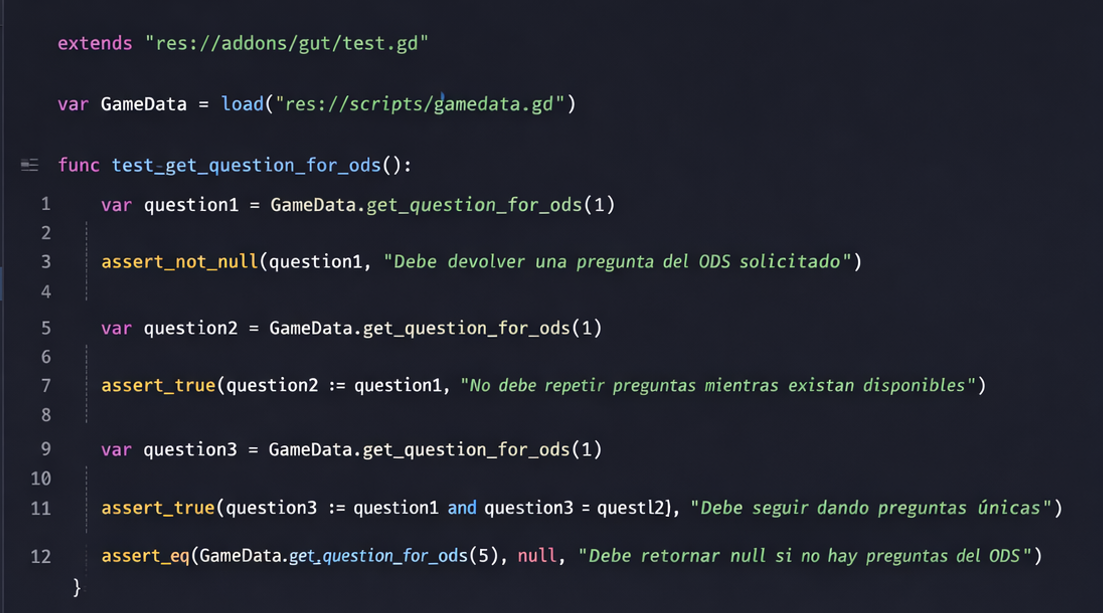
\includegraphics[width=0.9\textwidth]{Images/Caso de Prueba.png}
  \caption{Casos de prueba para la funcionalidad \texttt{get\_question\_for\_ods()} de la clase \texttt{GameData} (elaboración propia).\label{fig:casos_prueba_unitarias}}
\end{figure}

La figura anterior muestra la implementación de los casos de prueba utilizando el framework GUT, donde se definen ocho escenarios diferentes que evalúan si el sistema devuelve preguntas del ODS solicitado, evita repeticiones mientras existan preguntas disponibles y reinicia correctamente el ciclo cuando se agota el conjunto cargado desde el banco en formato JSON. La ejecución automatizada de estas pruebas permite verificar que la lógica implementada responde correctamente ante cada uno de los casos planteados, tal como se evidencia en los resultados presentados a continuación.

\begin{figure}[H]
  \centering
  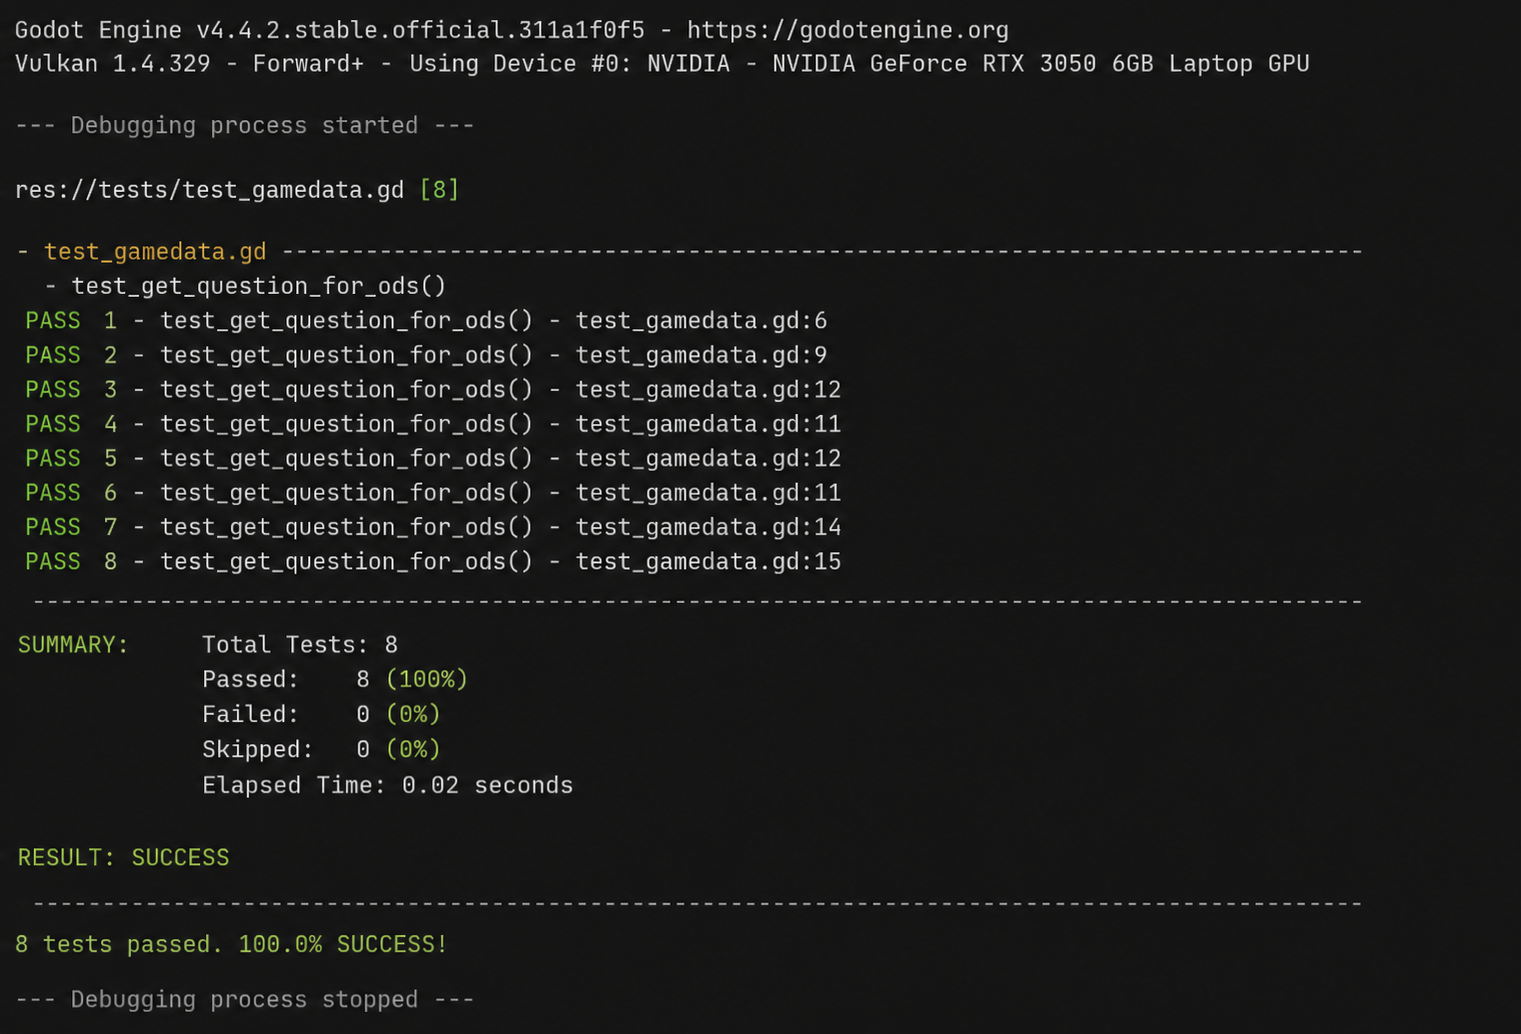
\includegraphics[width=0.6\textwidth]{Images/Resultado de Prueba.png}
  \caption{Resultado de pruebas para la clase \texttt{GameData} (elaboración propia).\label{fig:resultado_pruebas_unitarias}}
\end{figure}

Todas las funcionalidades probadas de esta forma pasaron las pruebas exitosamente, lo que no significa que no puedan existir defectos, ya que la interoperabilidad entre módulos puede causar problemas, lo que lleva a la necesidad de la aplicación de otro nivel de pruebas.

\subsection{Aplicación de pruebas de aceptación}
\label{subsec:aplicacion_pruebas_aceptacion}

Las pruebas de aceptación se realizaron siguiendo la metodología Extreme Programming, ejecutándose al finalizar cada una de las cinco iteraciones de desarrollo establecidas en el Capítulo 2. Esta organización permite validar incrementalmente el software conforme se implementan nuevas funcionalidades, detectando errores de forma temprana y asegurando que cada entrega parcial cumpla con los criterios de aceptación antes de proceder a la siguiente iteración.

Se ejecutaron un total de 18 casos de prueba vinculados a las historias de usuario implementadas para validar el cumplimiento de los criterios de aceptación establecidos. A continuación se presenta el caso de prueba correspondiente a la historia de usuario 9, que fue el único que presentó una no conformidad durante la Iteración 3. Los 17 casos de prueba restantes se encuentran detallados en el Anexo D.

\begin{table}[H]
\centering
\caption{Caso de prueba de aceptación \#9 Mostrar pregunta ODS (elaboración propia)\label{tab:cpa9}}
\renewcommand{\arraystretch}{1.3}
\begin{tabular}{|p{0.35\textwidth}|p{0.55\textwidth}|}
\hline
\multicolumn{2}{|c|}{\textbf{Caso de Prueba de Aceptación}} \\
\hline
\textbf{Código:} HU\#9\_PA\#1 & \textbf{Historia de Usuario:} 9 \\
\hline
\multicolumn{2}{|l|}{\textbf{Nombre:} Mostrar pregunta ODS} \\
\hline
\multicolumn{2}{|p{0.9\textwidth}|}{\textbf{Descripción:} Prueba realizada para verificar que al caer en una casilla ODS se muestre correctamente el panel de preguntas.} \\
\hline
\textbf{Pasos de ejecución:} & 1. Se mueve la ficha hasta una casilla ODS. \newline 2. Se verifica que aparezca el panel de preguntas. \newline 3. Se verifica que se muestren la pregunta y las opciones de respuesta. \\
\hline
\multicolumn{2}{|c|}{\textbf{Resultado:} No satisfactorio} \\
\hline
\end{tabular}
\end{table}

\subsubsection{Resultados de las pruebas de aceptación}

En las pruebas de aceptación se realizaron un total de 18 casos de prueba distribuidos en cinco iteraciones, obteniendo resultados mayormente positivos que evidencian la atención a los detalles críticos y la prevención de errores durante el proceso de implementación.

Los casos de prueba aplicados a las Iteraciones 1, 2, 4 y 5 dieron como resultado un 100\% de aprobación y 0\% de no conformidades, validando satisfactoriamente las funcionalidades base del videojuego, las mecánicas básicas de juego, las funcionalidades de cierre y las características complementarias. Sin embargo, en la Iteración 3 se detectó una no conformidad en el caso de prueba correspondiente a la historia de usuario 9 (Mostrar pregunta ODS), dando como resultado un 66.67\% de satisfacción y 33.33\% de insatisfacción para dicha iteración.

La no conformidad identificada consistió en un error de visualización en el panel de preguntas ODS, donde el texto de las opciones de respuesta se superponía con los bordes del panel cuando las respuestas contenían más de 50 caracteres, afectando la legibilidad y la experiencia de usuario. Este problema se presentaba específicamente en preguntas relacionadas con los ODS 8 (Trabajo decente y crecimiento económico) y ODS 16 (Paz, justicia e instituciones sólidas), cuyos enunciados tienden a ser más extensos.

Al corregir el error mediante el ajuste del tamaño de fuente y la implementación de saltos de línea automáticos en el componente de texto, y realizar nuevamente el caso de prueba a la historia de usuario 9, se obtuvo un resultado satisfactorio, elevando la Iteración 3 a un 100\% de aprobación. Tras esta corrección, se ejecutaron nuevamente todos los casos de prueba de las cinco iteraciones, confirmando que el videojuego \textit{Go Goals! Digital} cumple satisfactoriamente con todos los criterios de aceptación establecidos.

\subsection{Aplicación de pruebas de índice de aceptación}
\label{subsec:aplicacion_pruebas_indice}

Para la aplicación de esta prueba se contó con una muestra de diez jóvenes estudiantes de La Habana, con edades comprendidas entre 15 y 25 años, a los que se les distribuyó el videojuego \textit{Go Goals! Digital} para su evaluación. A dicha muestra se le administró un cuestionario estructurado, elaborado y diseñado específicamente para evaluar los criterios de aceptación.

\begin{table}[htbp]
\centering
\caption{Listado de estudiantes evaluadores (elaboración propia).\label{tab:probadores_beta}}
\renewcommand{\arraystretch}{1.3}
\begin{tabular}{|l|c|}
\hline
\textbf{Nombre y Apellidos} & \textbf{Edad} \\
\hline
José Miguel Martín Monzón & 18 \\
\hline
Oscar Raúl García Almestro & 22 \\
\hline
Royciel Chavez Garcés & 19 \\
\hline
Javier Ernesto Perdomo Batista & 24 \\
\hline
Yslen Marturelo Lorenzo & 16 \\
\hline
Janys Lourdes Cañizares de la Rosa & 21 \\
\hline
Pedro Luis Hernández Soto & 17 \\
\hline
Sofía Martínez Delgado & 25 \\
\hline
Carlos Alberto Ramos Pérez & 15 \\
\hline
Daniela Fernández Suárez & 20 \\
\hline
\end{tabular}
\end{table}

El cuestionario presentó la siguiente estructura:

\begin{longtable}{|p{0.95\textwidth}|}
\caption{Cuestionario de Satisfacción del Usuario -- Go Goals! Digital (elaboración propia).\label{tab:cuestionario_satisfaccion}} \\
\hline
\multicolumn{1}{|c|}{\textbf{Cuestionario de Satisfacción del Usuario -- Go Goals! Digital}} \\
\hline
\endfirsthead
\multicolumn{1}{c}
{{ \tablename\ \thetable{} -- Continuación de la página anterior}} \\
\hline
\multicolumn{1}{|c|}{\textbf{Cuestionario de Satisfacción del Usuario -- Go Goals! Digital}} \\
\hline
\endhead
\hline
\endfoot
\endlastfoot

\textbf{Instrucciones:} Por favor, responde cada pregunta considerando la siguiente escala de Likert:

1: Muy insatisfecho/a

2: Insatisfecho/a

3: Neutral

4: Satisfecho/a

5: Muy satisfecho/a \\
\hline
\multicolumn{1}{|c|}{\textbf{Sección 1: Experiencia General y Jugabilidad}} \\
\hline
\textbf{Jugabilidad General:}

¿Qué tan satisfecho/a estás con la jugabilidad general del videojuego? \\
\hline
\textbf{Control y Mecánicas:}

¿Qué tan intuitivas te resultan las mecánicas de control (lanzar dado, mover fichas, responder preguntas) en el juego? \\
\hline
\textbf{Desafíos y Equilibrio:}

¿Consideras que el nivel de desafío de las preguntas es adecuado para tu edad? \\
\hline
\multicolumn{1}{|c|}{\textbf{Sección 2: Interfaz y Diseño Visual}} \\
\hline
\textbf{Usabilidad e Interfaz:}

¿Qué tan clara e intuitiva es la interfaz del videojuego?

¿Qué tan útil te han resultado los tutoriales y elementos de ayuda integrados? \\
\hline
\textbf{Estética y Diseño Gráfico:}

¿Qué tan atractivo y coherente encuentras el diseño visual y la estética general del videojuego? \\
\hline
\multicolumn{1}{|c|}{\textbf{Sección 3: Rendimiento Técnico}} \\
\hline
\textbf{Rendimiento del Sistema:}

¿Estás satisfecho/a con el desempeño técnico del juego en términos de tiempos de carga, estabilidad y fluidez durante la experiencia de juego? \\
\hline
\multicolumn{1}{|c|}{\textbf{Sección 4: Contenido Educativo y Relación con los ODS}} \\
\hline
\textbf{Integración de Contenido Educativo:}

¿Qué tan claro y efectivo es el contenido relacionado con los Objetivos de Desarrollo Sostenible (ODS) dentro del videojuego? \\
\hline
\textbf{Impacto Educativo:}

¿Crees que el contenido del juego te ha motivado a informarte o reflexionar sobre temas de sostenibilidad? \\
\hline
\textbf{Balance entre Entretenimiento y Educación:}

¿Consideras que el juego logra un buen equilibrio entre ser entretenido y cumplir con su función educativa en cuanto a la promoción de los ODS? \\
\hline
\multicolumn{1}{|c|}{\textbf{Sección 5: Satisfacción Global y Recomendación}} \\
\hline
\textbf{Satisfacción Global:}

En general, ¿qué tan satisfecho/a estás con tu experiencia en \textit{Go Goals! Digital}? \\
\hline
\textbf{Recomendación:}

¿Recomendarías este videojuego a otras personas interesadas en videojuegos educativos o en sostenibilidad? (Opciones: Sí / No) \\
\hline
\end{longtable}

Al aplicarlo se obtuvieron resultados altamente positivos, con todos los usuarios recomendando probar el videojuego.
\begin{table}[H]
\centering
\caption{Resultados del cuestionario de satisfacción (elaboración propia).\label{tab:resultados_cuestionario}}
\renewcommand{\arraystretch}{1.3}
\begin{tabular}{|l|c|c|c|}
\hline
\textbf{Categoría} & \textbf{Respuestas positivas} & \textbf{Respuestas neutrales} & \textbf{Respuestas negativas} \\
\hline
Experiencia General y Jugabilidad & 30 & 0 & 0 \\
\hline
Interfaz y Diseño Visual & 28 & 2 & 0 \\
\hline
Rendimiento Técnico & 10 & 0 & 0 \\
\hline
Contenido Educativo y ODS & 30 & 0 & 0 \\
\hline
Satisfacción Global & 10 & 0 & 0 \\
\hline
\textbf{Total} & \textbf{108} & \textbf{2} & \textbf{0} \\
\hline
\end{tabular}
\end{table}

Tomando estos resultados se aplica la fórmula del CSAT, donde se divide el número de respuestas positivas entre el total de respuestas y se multiplica por 100. Al aplicar esta métrica se obtiene un cociente de 108 respuestas positivas dividido entre 110 respuestas totales que, al ser multiplicado por 100, resulta en 98.18\%. Este valor se considera extremadamente alto y valida objetivamente la calidad técnica, el diseño instruccional y la aceptación del videojuego educativo \textit{Go Goals! Digital} por parte de su público objetivo.

%---------------------------------------------------------------------------
\section*{Conclusiones del capítulo}

El diseño estructurado de la validación permitió asegurar una alta calidad en el proceso evaluativo, siguiendo las buenas prácticas de la metodología Extreme Programming. A través de la aplicación de pruebas unitarias automatizadas se garantizó el correcto funcionamiento de los módulos lógicos internos sin dependencias externas, previniendo defectos de integración. Las pruebas de aceptación validaron el videojuego en su totalidad desde la perspectiva de los usuarios finales. Finalmente, el índice de aceptación del 98.18\% documentado mediante el instrumento CSAT confirma que \textit{Go Goals! Digital} cumple satisfactoriamente con los objetivos pedagógicos y lúdicos planteados, resultando en un producto tecnológico altamente valorado por su público objetivo.

  \conclusions

Con el desarrollo del videojuego educativo \textit{Go Goals! Digital} se comprueba y reafirma el éxito y cumplimiento del propósito de esta investigación, obteniendo una solución a todas las problemáticas planteadas y abriendo la puerta a la innovación en el ámbito de los videojuegos educativos enfocados en la promoción de los Objetivos de Desarrollo Sostenible. El proceso de investigación y el análisis completo de la solución propuesta han permitido llegar a las siguientes conclusiones:

\begin{itemize}
    \item El marco teórico sobre videojuegos educativos, aprendizaje basado en juegos y gamificación demuestra el potencial pedagógico de estas herramientas en la educación para el desarrollo sostenible.
    
    \item El análisis de soluciones homólogas proporcionó patrones de diseño y mecánicas de juego que sirvieron como referencia en el desarrollo del sistema, identificando prácticas que debían evitarse para garantizar el éxito de la investigación.
    
    \item La definición de requisitos funcionales y no funcionales ayudó a establecer la estructura técnica y visual de la solución y garantizar una mayor comprensión del videojuego a desarrollar.
    
    \item El proceso de implementación da como resultado el sistema deseado que cumple con todas las especificaciones técnicas planteadas, además de contar con una estructura sólida desde su base metodológica hasta su arquitectura de desarrollo.
    
    \item Las pruebas realizadas después del desarrollo confirman que \textit{Go Goals! Digital} cumple con todas las expectativas y puede ser calificado como un videojuego educativo versátil, útil y necesario.
\end{itemize}
  \suggestions

A partir de los resultados obtenidos y de las proyecciones tecnológicas identificadas durante el ciclo de desarrollo, se proponen las siguientes líneas de trabajo futuro:

Se sugiere expandir el banco de preguntas relacionadas con los Objetivos de Desarrollo Sostenible, mediante la incorporación de múltiples niveles de complejidad cognitiva que doten al sistema de una mayor adaptabilidad para interactuar con diferentes grupos etarios.

Resulta pertinente implementar un sistema de logros y recompensas virtuales que fortalezca el paradigma de gamificación, de modo que se logre un mayor incentivo para que los jugadores completen desafíos específicos y asimilen el contenido de sostenibilidad a largo plazo.

Se exhorta a diseñar una arquitectura de red para habilitar un modo multijugador en línea, lo cual permitiría la interconexión de estudiantes de diferentes instituciones escolares y promovería el intercambio dinámico de conocimientos.

Se recomienda enriquecer el diseño visual del proyecto mediante la adición de microanimaciones y efectos de transición de turnos elaborados, maximizando la inmersión de la experiencia de juego.

Finalmente, se propone refactorizar la vista y los controles del sistema para su distribución nativa en plataformas móviles, lo que permitiría ampliar drásticamente el alcance y la accesibilidad del recurso educativo en la población.

  \appendixes

\begin{addendum}
	%\chapter{Proyectos y Avales}
    %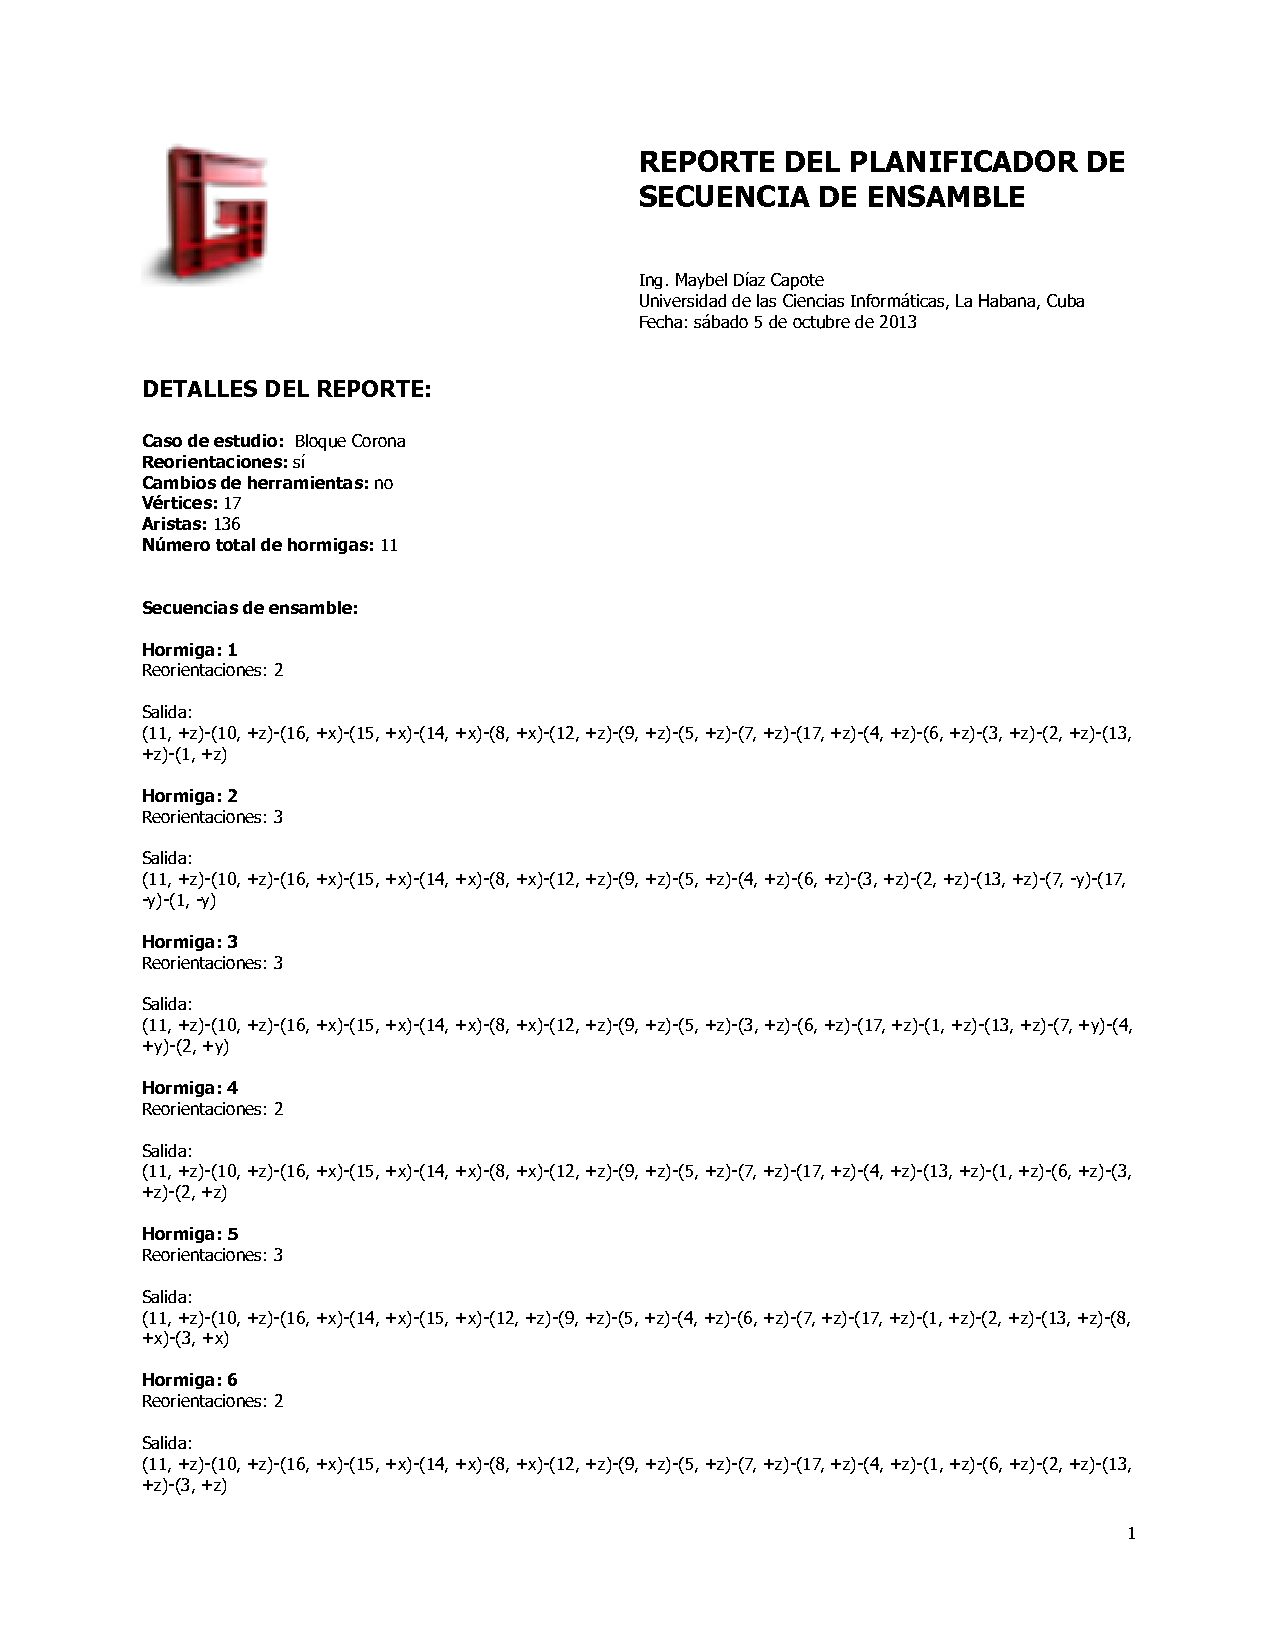
\includegraphics[scale=0.45]{Anexos/BloqueCoronaReport}
   
  	%\chapter{Otro reporte}
  	%\section{Otra sección de muestra}
  	%De una sola \hypertarget{word}{sentencia} 
	%\section{Otro ensamble Industrial}
	%\label{anx:ensambleindustrial}
	%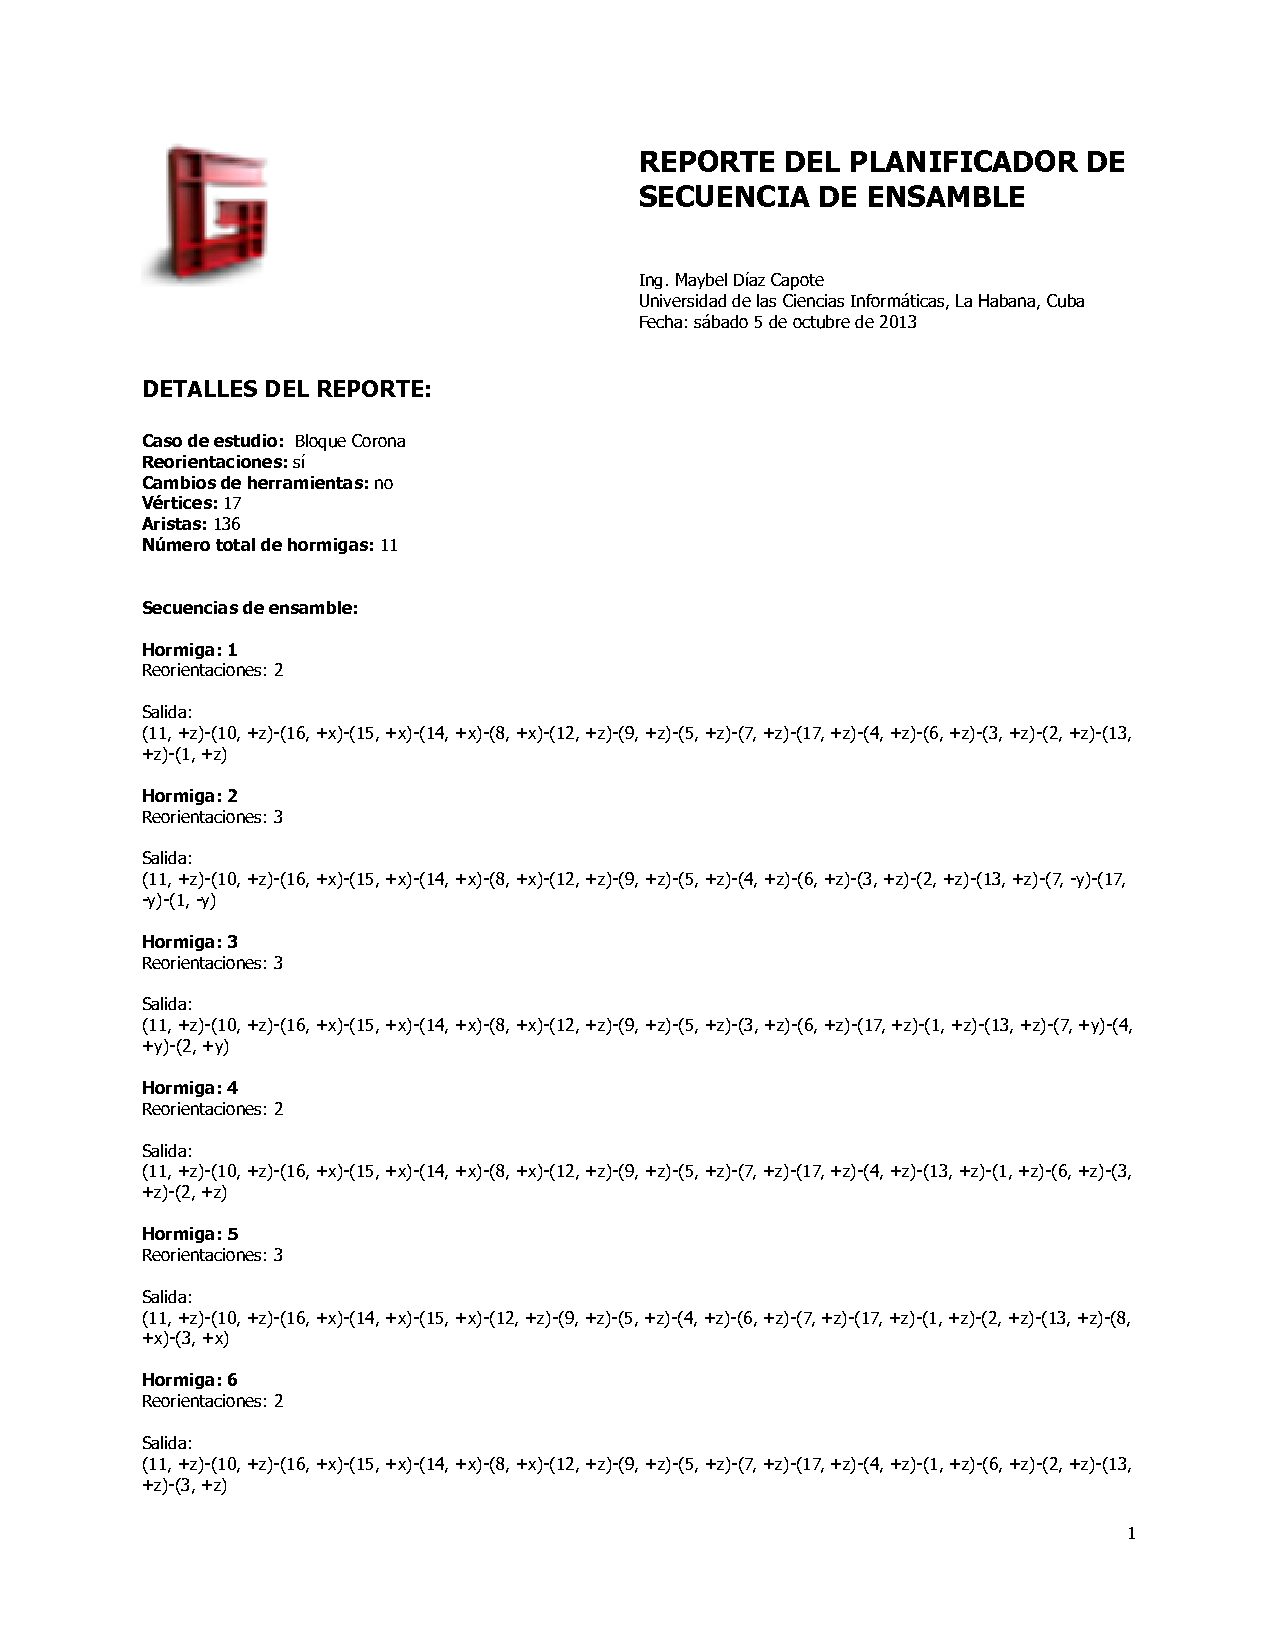
\includegraphics[scale=0.45]{Anexos/BloqueCoronaReport}
	\chapter{Historias de Usuario}
	\label{anx:historias_usuario}
	
	\begin{table}[H]
\centering
\caption{Historia de usuario 1: Mostrar menú principal (elaboración propia).\label{tab:hu1}}
\renewcommand{\arraystretch}{1.5}
\begin{tabular}{|p{0.45\textwidth}|p{0.45\textwidth}|}
\hline
\multicolumn{2}{|l|}{\textbf{Historia de Usuario}} \\
\hline
\textbf{Número:} 1 & \textbf{Nombre:} Mostrar menú principal \\
\hline
\textbf{Prioridad:} Alta & \textbf{Riesgo:} Baja \\
\hline
\textbf{Puntos de estimación:} 1.0 & \textbf{Iteración asignada:} 1 \\
\hline
\multicolumn{2}{|p{0.945\textwidth}|}{\textbf{Descripción:} Como usuario quiero acceder a un menú principal intuitivo para navegar por las opciones principales del juego.} \\
\hline
\multicolumn{2}{|p{0.945\textwidth}|}{\textbf{Observaciones:}
\vspace{-0.5em}
\begin{itemize}
    \setlength\itemsep{0em}
    \item El menú principal debe incluir botones: Iniciar Partida, Instrucciones y Salir.
\end{itemize}
\vspace{-1em}
} \\
\hline
\end{tabular}
\end{table}

\begin{table}[H]
\centering
\caption{Historia de usuario 2: Mostrar pantalla de instrucciones (elaboración propia).\label{tab:hu2}}
\renewcommand{\arraystretch}{1.5}
\begin{tabular}{|p{0.45\textwidth}|p{0.45\textwidth}|}
\hline
\multicolumn{2}{|l|}{\textbf{Historia de Usuario}} \\
\hline
\textbf{Número:} 2 & \textbf{Nombre:} Mostrar pantalla de instrucciones \\
\hline
\textbf{Prioridad:} Media & \textbf{Riesgo:} Baja \\
\hline
\textbf{Puntos de estimación:} 1.0 & \textbf{Iteración asignada:} 1 \\
\hline
\multicolumn{2}{|p{0.945\textwidth}|}{\textbf{Descripción:} Como jugador quiero leer las instrucciones del juego para aprender a jugarlo correctamente.} \\
\hline
\multicolumn{2}{|p{0.945\textwidth}|}{\textbf{Observaciones:}
\vspace{-0.5em}
\begin{itemize}
    \setlength\itemsep{0em}
    \item La pantalla debe explicar las reglas de avance, escalera, serpiente y preguntas ODS de forma visual.
    \item Debe ser accesible desde el menú principal.
\end{itemize}
\vspace{-1em}
} \\
\hline
\end{tabular}
\end{table}

\begin{table}[H]
\centering
\caption{Historia de usuario 3: Iniciar partida (elaboración propia).\label{tab:hu3}}
\renewcommand{\arraystretch}{1.5}
\begin{tabular}{|p{0.45\textwidth}|p{0.45\textwidth}|}
\hline
\multicolumn{2}{|l|}{\textbf{Historia de Usuario}} \\
\hline
\textbf{Número:} 3 & \textbf{Nombre:} Iniciar partida \\
\hline
\textbf{Prioridad:} Alta & \textbf{Riesgo:} Medio \\
\hline
\textbf{Puntos de estimación:} 2.0 & \textbf{Iteración asignada:} 1 \\
\hline
\multicolumn{2}{|p{0.945\textwidth}|}{\textbf{Descripción:} Como jugador quiero iniciar una nueva partida para aprender sobre los ODS de manera interactiva.} \\
\hline
\multicolumn{2}{|p{0.945\textwidth}|}{\textbf{Observaciones:}
\vspace{-0.5em}
\begin{itemize}
    \setlength\itemsep{0em}
    \item Debe incluir botón para iniciar partida.
    \item Permite configurar número de jugadores (1--4).
    \item Carga el tablero y realiza transición a la primera ronda.
    \item Se inicializan estadísticas en cero.
\end{itemize}
\vspace{-1em}
} \\
\hline
\end{tabular}
\end{table}

\begin{table}[H]
\centering
\caption{Historia de usuario 4: Visualizar tablero (elaboración propia).\label{tab:hu4}}
\renewcommand{\arraystretch}{1.5}
\begin{tabular}{|p{0.45\textwidth}|p{0.45\textwidth}|}
\hline
\multicolumn{2}{|l|}{\textbf{Historia de Usuario}} \\
\hline
\textbf{Número:} 4 & \textbf{Nombre:} Visualizar tablero \\
\hline
\textbf{Prioridad:} Alta & \textbf{Riesgo:} Alto \\
\hline
\textbf{Puntos de estimación:} 5.0 & \textbf{Iteración asignada:} 1 \\
\hline
\multicolumn{2}{|p{0.945\textwidth}|}{\textbf{Descripción:} Como jugador quiero ver el tablero completo de 63 casillas para entender el recorrido hacia el año 2030.} \\
\hline
\multicolumn{2}{|p{0.945\textwidth}|}{\textbf{Observaciones:}
\vspace{-0.5em}
\begin{itemize}
    \setlength\itemsep{0em}
    \item El tablero debe ser fiel al diseño oficial.
    \item Las 17 casillas temáticas deben identificarse con el ícono del ODS correspondiente.
    \item El tablero debe ser visible sin \textit{scroll}.
    \item Debe ser adaptable a distintas resoluciones de pantalla.
\end{itemize}
\vspace{-1em}
} \\
\hline
\end{tabular}
\end{table}

\begin{table}[H]
\centering
\caption{Historia de usuario 5: Lanzar dado (elaboración propia).\label{tab:hu5}}
\renewcommand{\arraystretch}{1.5}
\begin{tabular}{|p{0.45\textwidth}|p{0.45\textwidth}|}
\hline
\multicolumn{2}{|l|}{\textbf{Historia de Usuario}} \\
\hline
\textbf{Número:} 5 & \textbf{Nombre:} Lanzar dado \\
\hline
\textbf{Prioridad:} Alta & \textbf{Riesgo:} Medio \\
\hline
\textbf{Puntos de estimación:} 1.5 & \textbf{Iteración asignada:} 2 \\
\hline
\multicolumn{2}{|p{0.945\textwidth}|}{\textbf{Descripción:} Como jugador quiero lanzar un dado virtual para determinar el avance de mi ficha en el tablero.} \\
\hline
\multicolumn{2}{|p{0.945\textwidth}|}{\textbf{Observaciones:}
\vspace{-0.5em}
\begin{itemize}
    \setlength\itemsep{0em}
    \item Debe mostrar animación breve del dado.
    \item El resultado entre 1 y 6 debe ser pseudoaleatorio.
    \item No debe ser posible lanzar el dado más de una vez por turno.
    \item Debe incluir \textit{feedback} visual y sonoro al obtener el resultado.
\end{itemize}
\vspace{-1em}
} \\
\hline
\end{tabular}
\end{table}

\begin{table}[H]
\centering
\caption{Historia de usuario 6: Mover ficha (elaboración propia).\label{tab:hu6}}
\renewcommand{\arraystretch}{1.5}
\begin{tabular}{|p{0.45\textwidth}|p{0.45\textwidth}|}
\hline
\multicolumn{2}{|l|}{\textbf{Historia de Usuario}} \\
\hline
\textbf{Número:} 6 & \textbf{Nombre:} Mover ficha \\
\hline
\textbf{Prioridad:} Alta & \textbf{Riesgo:} Alto \\
\hline
\textbf{Puntos de estimación:} 4.0 & \textbf{Iteración asignada:} 2 \\
\hline
\multicolumn{2}{|p{0.945\textwidth}|}{\textbf{Descripción:} Como jugador quiero que mi ficha se mueva automáticamente según el resultado del dado para concentrarme en el contenido educativo.} \\
\hline
\multicolumn{2}{|p{0.945\textwidth}|}{\textbf{Observaciones:}
\vspace{-0.5em}
\begin{itemize}
    \setlength\itemsep{0em}
    \item El movimiento debe ser animado casilla por casilla.
    \item Debe calcularse la trayectoria correcta.
    \item Al llegar a la casilla final se comprueba si es casilla ODS, escalera o serpiente.
\end{itemize}
\vspace{-1em}
} \\
\hline
\end{tabular}
\end{table}

\begin{table}[H]
\centering
\caption{Historia de usuario 7: Aplicar efecto de escalera (elaboración propia).\label{tab:hu7}}
\renewcommand{\arraystretch}{1.5}
\begin{tabular}{|p{0.45\textwidth}|p{0.45\textwidth}|}
\hline
\multicolumn{2}{|l|}{\textbf{Historia de Usuario}} \\
\hline
\textbf{Número:} 7 & \textbf{Nombre:} Aplicar efecto de escalera \\
\hline
\textbf{Prioridad:} Alta & \textbf{Riesgo:} Medio \\
\hline
\textbf{Puntos de estimación:} 1.5 & \textbf{Iteración asignada:} 2 \\
\hline
\multicolumn{2}{|p{0.945\textwidth}|}{\textbf{Descripción:} Como jugador quiero que mi ficha avance automáticamente por una escalera al caer en su base para ser recompensado por mi progreso.} \\
\hline
\multicolumn{2}{|p{0.945\textwidth}|}{\textbf{Observaciones:}
\vspace{-0.5em}
\begin{itemize}
    \setlength\itemsep{0em}
    \item El sistema debe detectar si la casilla final es la base de una escalera.
    \item La ficha debe avanzar a la casilla destino con animación de subida.
    \item Debe incluir \textit{feedback} sonoro positivo.
\end{itemize}
\vspace{-1em}
} \\
\hline
\end{tabular}
\end{table}

\begin{table}[H]
\centering
\caption{Historia de usuario 8: Aplicar efecto de serpiente (elaboración propia).\label{tab:hu8}}
\renewcommand{\arraystretch}{1.5}
\begin{tabular}{|p{0.45\textwidth}|p{0.45\textwidth}|}
\hline
\multicolumn{2}{|l|}{\textbf{Historia de Usuario}} \\
\hline
\textbf{Número:} 8 & \textbf{Nombre:} Aplicar efecto de serpiente \\
\hline
\textbf{Prioridad:} Alta & \textbf{Riesgo:} Medio \\
\hline
\textbf{Puntos de estimación:} 1.5 & \textbf{Iteración asignada:} 2 \\
\hline
\multicolumn{2}{|p{0.945\textwidth}|}{\textbf{Descripción:} Como jugador quiero que mi ficha retroceda automáticamente al caer en la cabeza de una serpiente para aplicar la penalización del juego clásico.} \\
\hline
\multicolumn{2}{|p{0.945\textwidth}|}{\textbf{Observaciones:}
\vspace{-0.5em}
\begin{itemize}
    \setlength\itemsep{0em}
    \item El sistema debe detectar si la casilla final es la cabeza de una serpiente.
    \item La ficha retrocede a la casilla destino con animación descendente.
    \item Debe incluir \textit{feedback} sonoro negativo.
\end{itemize}
\vspace{-1em}
} \\
\hline
\end{tabular}
\end{table}

\begin{table}[H]
\centering
\caption{Historia de usuario 10: Evaluar respuesta (elaboración propia).\label{tab:hu10}}
\renewcommand{\arraystretch}{1.5}
\begin{tabular}{|p{0.45\textwidth}|p{0.45\textwidth}|}
\hline
\multicolumn{2}{|l|}{\textbf{Historia de Usuario}} \\
\hline
\textbf{Número:} 10 & \textbf{Nombre:} Evaluar respuesta \\
\hline
\textbf{Prioridad:} Alta & \textbf{Riesgo:} Medio \\
\hline
\textbf{Puntos de estimación:} 3.0 & \textbf{Iteración asignada:} 3 \\
\hline
\multicolumn{2}{|p{0.945\textwidth}|}{\textbf{Descripción:} Como jugador quiero recibir retroalimentación inmediata al responder para entender si acerté y por qué.} \\
\hline
\multicolumn{2}{|p{0.945\textwidth}|}{\textbf{Observaciones:}
\vspace{-0.5em}
\begin{itemize}
    \setlength\itemsep{0em}
    \item El sistema debe mostrar un indicador visual de resultado (verde/rojo).
    \item Debe mostrar un mensaje explicativo breve de la respuesta correcta.
    \item Si la respuesta es correcta, el jugador recibe una bonificación obteniendo la oportunidad de volver a lanzar los dados. Si es incorrecta, el turno finaliza y pasa al siguiente jugador.
\end{itemize}
\vspace{-1em}
} \\
\hline
\end{tabular}
\end{table}

\begin{table}[H]
\centering
\caption{Historia de usuario 11: Gestionar turnos (elaboración propia).\label{tab:hu11}}
\renewcommand{\arraystretch}{1.5}
\begin{tabular}{|p{0.45\textwidth}|p{0.45\textwidth}|}
\hline
\multicolumn{2}{|l|}{\textbf{Historia de Usuario}} \\
\hline
\textbf{Número:} 11 & \textbf{Nombre:} Gestionar turnos \\
\hline
\textbf{Prioridad:} Alta & \textbf{Riesgo:} Baja \\
\hline
\textbf{Puntos de estimación:} 2.0 & \textbf{Iteración asignada:} 3 \\
\hline
\multicolumn{2}{|p{0.945\textwidth}|}{\textbf{Descripción:} Como jugador quiero que el sistema gestione turnos automáticamente y muestre quién es el jugador activo para que el juego fluya.} \\
\hline
\multicolumn{2}{|p{0.945\textwidth}|}{\textbf{Observaciones:}
\vspace{-0.5em}
\begin{itemize}
    \setlength\itemsep{0em}
    \item El sistema debe indicar visualmente el jugador activo resaltando su ficha.
    \item Al finalizar el turno debe pasar automáticamente al siguiente jugador en orden.
\end{itemize}
\vspace{-1em}
} \\
\hline
\end{tabular}
\end{table}

\begin{table}[H]
\centering
\caption{Historia de usuario 12: Determinar condición de victoria (elaboración propia).\label{tab:hu12}}
\renewcommand{\arraystretch}{1.5}
\begin{tabular}{|p{0.45\textwidth}|p{0.45\textwidth}|}
\hline
\multicolumn{2}{|l|}{\textbf{Historia de Usuario}} \\
\hline
\textbf{Número:} 12 & \textbf{Nombre:} Determinar condición de victoria \\
\hline
\textbf{Prioridad:} Alta & \textbf{Riesgo:} Baja \\
\hline
\textbf{Puntos de estimación:} 1.5 & \textbf{Iteración asignada:} 4 \\
\hline
\multicolumn{2}{|p{0.945\textwidth}|}{\textbf{Descripción:} Como jugador quiero que el juego detecte cuando alguien llegue a la casilla 63 para mostrar la pantalla de victoria.} \\
\hline
\multicolumn{2}{|p{0.945\textwidth}|}{\textbf{Observaciones:}
\vspace{-0.5em}
\begin{itemize}
    \setlength\itemsep{0em}
    \item El sistema debe detectar la llegada exacta a la casilla final.
    \item Debe mostrar una pantalla de victoria con animación de confeti y el nombre del ganador.
\end{itemize}
\vspace{-1em}
} \\
\hline
\end{tabular}
\end{table}

\begin{table}[H]
\centering
\caption{Historia de usuario 13: Mostrar estadísticas de partida (elaboración propia).\label{tab:hu13}}
\renewcommand{\arraystretch}{1.5}
\begin{tabular}{|p{0.45\textwidth}|p{0.45\textwidth}|}
\hline
\multicolumn{2}{|l|}{\textbf{Historia de Usuario}} \\
\hline
\textbf{Número:} 13 & \textbf{Nombre:} Mostrar estadísticas de partida \\
\hline
\textbf{Prioridad:} Media & \textbf{Riesgo:} Medio \\
\hline
\textbf{Puntos de estimación:} 4.0 & \textbf{Iteración asignada:} 4 \\
\hline
\multicolumn{2}{|p{0.945\textwidth}|}{\textbf{Descripción:} Como educador quiero visualizar estadísticas de desempeño por jugador y por ODS de manera continua en tiempo real para evaluar el aprendizaje progresivamente.} \\
\hline
\multicolumn{2}{|p{0.945\textwidth}|}{\textbf{Observaciones:}
\vspace{-0.5em}
\begin{itemize}
    \setlength\itemsep{0em}
    \item Debe existir una interfaz accesible que muestre las estadísticas de desempeño de cada jugador en tiempo real.
    \item Debe incluir el porcentaje de respuestas correctas por jugador.
    \item Debe identificar los ODS con menor porcentaje de aciertos para cada jugador.
\end{itemize}
\vspace{-1em}
} \\
\hline
\end{tabular}
\end{table}

\begin{table}[H]
\centering
\caption{Historia de usuario 14: Configurar audio (elaboración propia).\label{tab:hu14}}
\renewcommand{\arraystretch}{1.5}
\begin{tabular}{|p{0.45\textwidth}|p{0.45\textwidth}|}
\hline
\multicolumn{2}{|l|}{\textbf{Historia de Usuario}} \\
\hline
\textbf{Número:} 14 & \textbf{Nombre:} Configurar audio \\
\hline
\textbf{Prioridad:} Baja & \textbf{Riesgo:} Baja \\
\hline
\textbf{Puntos de estimación:} 2.5 & \textbf{Iteración asignada:} 4 \\
\hline
\multicolumn{2}{|p{0.945\textwidth}|}{\textbf{Descripción:} Como jugador quiero poder activar o desactivar la música y los efectos de sonido para personalizar mi partida.} \\
\hline
\multicolumn{2}{|p{0.945\textwidth}|}{\textbf{Observaciones:}
\vspace{-0.5em}
\begin{itemize}
    \setlength\itemsep{0em}
    \item Debe incluir controles para el volumen global, música y efectos sonoros.
\end{itemize}
\vspace{-1em}
} \\
\hline
\end{tabular}
\end{table}

\begin{table}[H]
\centering
\caption{Historia de usuario 15: Pausar partida (elaboración propia).\label{tab:hu15}}
\renewcommand{\arraystretch}{1.5}
\begin{tabular}{|p{0.45\textwidth}|p{0.45\textwidth}|}
\hline
\multicolumn{2}{|l|}{\textbf{Historia de Usuario}} \\
\hline
\textbf{Número:} 15 & \textbf{Nombre:} Pausar partida \\
\hline
\textbf{Prioridad:} Media & \textbf{Riesgo:} Baja \\
\hline
\textbf{Puntos de estimación:} 1.0 & \textbf{Iteración asignada:} 4 \\
\hline
\multicolumn{2}{|p{0.945\textwidth}|}{\textbf{Descripción:} Como jugador quiero pausar la partida en cualquier momento para atender interrupciones sin perder el progreso.} \\
\hline
\multicolumn{2}{|p{0.945\textwidth}|}{\textbf{Observaciones:}
\vspace{-0.5em}
\begin{itemize}
    \setlength\itemsep{0em}
    \item Debe existir un panel de pausa que detenga todo el flujo y las animaciones.
    \item Debe permitir reanudar desde el estado exacto en que se pausó.
\end{itemize}
\vspace{-1em}
} \\
\hline
\end{tabular}
\end{table}

\begin{table}[H]
\centering
\caption{Historia de usuario 16: Reiniciar partida (elaboración propia).\label{tab:hu16}}
\renewcommand{\arraystretch}{1.5}
\begin{tabular}{|p{0.45\textwidth}|p{0.45\textwidth}|}
\hline
\multicolumn{2}{|l|}{\textbf{Historia de Usuario}} \\
\hline
\textbf{Número:} 16 & \textbf{Nombre:} Reiniciar partida \\
\hline
\textbf{Prioridad:} Media & \textbf{Riesgo:} Baja \\
\hline
\textbf{Puntos de estimación:} 1.0 & \textbf{Iteración asignada:} 4 \\
\hline
\multicolumn{2}{|p{0.945\textwidth}|}{\textbf{Descripción:} Como jugador quiero reiniciar la partida actual desde cero sin tener que volver a configurar el número de jugadores.} \\
\hline
\multicolumn{2}{|p{0.945\textwidth}|}{\textbf{Observaciones:}
\vspace{-0.5em}
\begin{itemize}
    \setlength\itemsep{0em}
    \item Accesible desde el menú de pausa o de victoria.
    \item Debe restaurar las posiciones y vaciar las estadísticas de la sesión actual.
\end{itemize}
\vspace{-1em}
} \\
\hline
\end{tabular}
\end{table}

\begin{table}[H]
\centering
\caption{Historia de usuario 17: Habilitar cámara de seguimiento (elaboración propia).\label{tab:hu17}}
\renewcommand{\arraystretch}{1.5}
\begin{tabular}{|p{0.45\textwidth}|p{0.45\textwidth}|}
\hline
\multicolumn{2}{|l|}{\textbf{Historia de Usuario}} \\
\hline
\textbf{Número:} 17 & \textbf{Nombre:} Habilitar cámara de seguimiento \\
\hline
\textbf{Prioridad:} Alta & \textbf{Riesgo:} Medio \\
\hline
\textbf{Puntos de estimación:} 2.0 & \textbf{Iteración asignada:} 5 \\
\hline
\multicolumn{2}{|p{0.945\textwidth}|}{\textbf{Descripción:} Como jugador quiero que la cámara enfoque automáticamente a mi ficha cuando sea mi turno para tener mejor inmersión y saber que me toca.} \\
\hline
\multicolumn{2}{|p{0.945\textwidth}|}{\textbf{Observaciones:}
\vspace{-0.5em}
\begin{itemize}
    \setlength\itemsep{0em}
    \item La cámara debe realizar un \textit{zoom} suave y centrarse en el jugador activo al inicio de cada turno.
    \item Durante el movimiento de la ficha, la cámara debe seguir su trayectoria en tiempo real.
    \item Al finalizar el turno de un jugador, la cámara debe transicionar automáticamente hacia la ubicación de la ficha del siguiente jugador activo.
\end{itemize}
\vspace{-1em}
} \\
\hline
\end{tabular}
\end{table}

\begin{table}[H]
\centering
\caption{Historia de usuario 18: Habilitar modo de práctica (elaboración propia).\label{tab:hu18}}
\renewcommand{\arraystretch}{1.5}
\begin{tabular}{|p{0.45\textwidth}|p{0.45\textwidth}|}
\hline
\multicolumn{2}{|l|}{\textbf{Historia de Usuario}} \\
\hline
\textbf{Número:} 18 & \textbf{Nombre:} Habilitar modo de práctica \\
\hline
\textbf{Prioridad:} Media & \textbf{Riesgo:} Bajo \\
\hline
\textbf{Puntos de estimación:} 5.0 & \textbf{Iteración asignada:} 5 \\
\hline
\multicolumn{2}{|p{0.945\textwidth}|}{\textbf{Descripción:} Como usuario nuevo quiero poder jugar la partida completamente solo, recorriendo el tablero a mi propio ritmo para practicar y conocer mis habilidades.} \\
\hline
\multicolumn{2}{|p{0.945\textwidth}|}{\textbf{Observaciones:}
\vspace{-0.5em}
\begin{itemize}
    \setlength\itemsep{0em}
    \item El entorno conserva todo el ciclo de progreso, escaleras y rondas de preguntas educativas pero restringido y centrado únicamente en el desarrollo individual del jugador.
\end{itemize}
\vspace{-1em}
} \\
\hline
\end{tabular}
\end{table}


	\chapter{Tarjetas CRC}
	\label{anx:tarjetas_crc}
	
	\begin{table}[H]
\centering
\caption{Tarjeta CRC GameData (Autoload) (elaboración propia).\label{tab:crc_gamedata}}
\begin{tabular}{|p{0.25\textwidth}|p{0.64\textwidth}|}
\hline
\multicolumn{2}{|c|}{\textbf{Tarjeta CRC}} \\
\hline
\textbf{Clase:} & GameData \\
\hline
\textbf{Responsabilidades} & - mantener la configuración de la partida (número de jugadores) \\
& - cargar y servir el banco de preguntas desde \texttt{questions.json} \\
& - proveer preguntas aleatorias por ODS sin repetición \\
\hline
\textbf{Clases relacionadas} & GameManager \\
& BoardConfig \\
\hline
\end{tabular}
\end{table}

\begin{table}[H]
\centering
\caption{Tarjeta CRC GameEvents (Bus de Eventos) (elaboración propia).\label{tab:crc_gameevents}}
\begin{tabular}{|p{0.25\textwidth}|p{0.64\textwidth}|}
\hline
\multicolumn{2}{|c|}{\textbf{Tarjeta CRC}} \\
\hline
\textbf{Clase:} & GameEvents \\
\hline
\textbf{Responsabilidades} & - definir las se\~nales globales del sistema: \texttt{dice\_rolled}, \texttt{player\_moving}, \texttt{quiz\_started}, \texttt{quiz\_requested(ods\_id)}, \texttt{game\_won} \\
& - actuar como canal de comunicación desacoplado entre lógica y UI \\
\hline
\textbf{Clases relacionadas} & GameManager \\
& Scripts de UI \\
\hline
\end{tabular}
\end{table}

\begin{table}[H]
\centering
\caption{Tarjeta CRC GameState (elaboración propia).\label{tab:crc_gamestate}}
\begin{tabular}{|p{0.25\textwidth}|p{0.64\textwidth}|}
\hline
\multicolumn{2}{|c|}{\textbf{Tarjeta CRC}} \\
\hline
\textbf{Clase:} & GameState \\
\hline
\textbf{Responsabilidades} & - gestionar la fase activa del juego mediante enumeración (MENU, PLAYING, PAUSED, GAME\_OVER) \\
& - almacenar el estado de la partida en curso: jugador activo (\texttt{active\_player\_index}), posiciones y conteo de turnos \\
\hline
\textbf{Clases relacionadas} & GameManager \\
& Player \\
\hline
\end{tabular}
\end{table}

\begin{table}[H]
\centering
\caption{Tarjeta CRC BoardConfig (elaboración propia).\label{tab:crc_boardconfig}}
\begin{tabular}{|p{0.25\textwidth}|p{0.64\textwidth}|}
\hline
\multicolumn{2}{|c|}{\textbf{Tarjeta CRC}} \\
\hline
\textbf{Clase:} & BoardConfig \\
\hline
\textbf{Responsabilidades} & - definir la configuración estática del tablero: posiciones de escaleras, toboganes y casillas de pregunta por ODS \\
& - proveer información de tipo y destino de cada casilla \\
\hline
\textbf{Clases relacionadas} & GameManager \\
& Board \\
\hline
\end{tabular}
\end{table}

\begin{table}[H]
\centering
\caption{Tarjeta CRC Board (Entidad) (elaboración propia).\label{tab:crc_board}}
\begin{tabular}{|p{0.25\textwidth}|p{0.64\textwidth}|}
\hline
\multicolumn{2}{|c|}{\textbf{Tarjeta CRC}} \\
\hline
\textbf{Clase:} & Board \\
\hline
\textbf{Responsabilidades} & - representar el estado visual y lógico del tablero de 63 casillas \\
& - exponer métodos de acceso a posiciones específicas \\
\hline
\textbf{Clases relacionadas} & GameManager \\
& Tile \\
& BoardConfig \\
\hline
\end{tabular}
\end{table}

\begin{table}[H]
\centering
\caption{Tarjeta CRC Tile (Entidad) (elaboración propia).\label{tab:crc_tile}}
\begin{tabular}{|p{0.25\textwidth}|p{0.64\textwidth}|}
\hline
\multicolumn{2}{|c|}{\textbf{Tarjeta CRC}} \\
\hline
\textbf{Clase:} & Tile \\
\hline
\textbf{Responsabilidades} & - mantener el tipo de casilla (normal, escalera, tobogán, quiz, meta) \\
& - almacenar el destino de traslado en caso de casilla especial \\
& - almacenar el identificador ODS en caso de casilla de pregunta \\
\hline
\textbf{Clases relacionadas} & Board \\
& GameManager \\
\hline
\end{tabular}
\end{table}

\begin{table}[H]
\centering
\caption{Tarjeta CRC Player (Entidad) (elaboración propia).\label{tab:crc_player}}
\begin{tabular}{|p{0.25\textwidth}|p{0.64\textwidth}|}
\hline
\multicolumn{2}{|c|}{\textbf{Tarjeta CRC}} \\
\hline
\textbf{Clase:} & Player \\
\hline
\textbf{Responsabilidades} & - mantener la posición actual y el historial de turnos del jugador \\
& - almacenar nombre e identificador de color de ficha \\
& - registrar estadísticas de respuestas \\
\hline
\textbf{Clases relacionadas} & GameState \\
& GameManager \\
\hline
\end{tabular}
\end{table}

\begin{table}[H]
\centering
\caption{Tarjeta CRC AudioManager (Autoload) (elaboración propia).\label{tab:crc_audiomanager}}
\begin{tabular}{|p{0.25\textwidth}|p{0.64\textwidth}|}
\hline
\multicolumn{2}{|c|}{\textbf{Tarjeta CRC}} \\
\hline
\textbf{Clase:} & AudioManager \\
\hline
\textbf{Responsabilidades} & - centralizar la reproducción de música de fondo y efectos de sonido \\
& - controlar el volumen global \\
& - liberar a los nodos de juego de gestionar \texttt{AudioStreamPlayer} locales \\
\hline
\textbf{Clases relacionadas} & GameManager \\
& Scripts de UI \\
\hline
\end{tabular}
\end{table}

\begin{table}[H]
\centering
\caption{Tarjeta CRC RecordsManager (Autoload) (elaboración propia).\label{tab:crc_recordsmanager}}
\begin{tabular}{|p{0.25\textwidth}|p{0.64\textwidth}|}
\hline
\multicolumn{2}{|c|}{\textbf{Tarjeta CRC}} \\
\hline
\textbf{Clase:} & RecordsManager \\
\hline
\textbf{Responsabilidades} & - gestionar la persistencia de puntuaciones y logros entre sesiones \\
& - proveer datos históricos para la pantalla de estadísticas \\
\hline
\textbf{Clases relacionadas} & GameManager \\
& Player \\
\hline
\end{tabular}
\end{table}


	\chapter{Tareas de Ingeniería}
	\label{anx:tareas_ingenieria}
	
	\begin{table}[H]
\centering
\caption{Tarea de ingeniería 1: Implementación del menú y pantalla de instrucciones (elaboración propia).\label{tab:ti1}}
\begin{tabular}{|p{0.3\textwidth}|p{0.65\textwidth}|}
\hline
\textbf{Campo} & \textbf{Descripción} \\
\hline
Tarea \# & 1 \\
\hline
HU relacionada & HU \#1, HU \#2 \\
\hline
Nombre & Implementación del menú principal y pantalla de instrucciones \\
\hline
Tipo & Desarrollo \\
\hline
Puntos estimados & 2.0 días \\
\hline
Iteración & 1 \\
\hline
Programador & Ruslan Alexei Martinez Campos \\
\hline
Descripción & Se diseñan las interfaces gráficas del menú principal y la pantalla de instrucciones en Godot, incluyendo navegación y elementos educativos. \\
\hline
\end{tabular}
\end{table}

\begin{table}[H]
\centering
\caption{Tarea de ingeniería 2: Visualización e inicio de partida (elaboración propia).\label{tab:ti2}}
\begin{tabular}{|p{0.3\textwidth}|p{0.65\textwidth}|}
\hline
\textbf{Campo} & \textbf{Descripción} \\
\hline
Tarea \# & 2 \\
\hline
HU relacionada & HU \#3, HU \#4 \\
\hline
Nombre & Visualización e inicio de partida \\
\hline
Tipo & Desarrollo \\
\hline
Puntos estimados & 7.0 días \\
\hline
Iteración & 1 \\
\hline
Programador & Ruslan Alexei Martinez Campos \\
\hline
Descripción & Se modela el tablero hexagonal de 63 casillas y se implementa la interfaz de configuración de partida para instanciar a los jugadores. \\
\hline
\end{tabular}
\end{table}

\begin{table}[H]
\centering
\caption{Tarea de ingeniería 3: Lógica del dado y movimiento de fichas (elaboración propia).\label{tab:ti3}}
\begin{tabular}{|p{0.3\textwidth}|p{0.65\textwidth}|}
\hline
\textbf{Campo} & \textbf{Descripción} \\
\hline
Tarea \# & 3 \\
\hline
HU relacionada & HU \#5, HU \#6 \\
\hline
Nombre & Implementación de la lógica del dado y movimiento animado \\
\hline
Tipo & Desarrollo \\
\hline
Puntos estimados & 5.5 días \\
\hline
Iteración & 2 \\
\hline
Programador & Ruslan Alexei Martinez Campos \\
\hline
Descripción & Se programa la lógica pseudoaleatoria del dado y se implementa el controlador para animar el recorrido de las fichas casilla a casilla. \\
\hline
\end{tabular}
\end{table}

\begin{table}[H]
\centering
\caption{Tarea de ingeniería 4: Lógica de efectos de casillas especiales (elaboración propia).\label{tab:ti4}}
\begin{tabular}{|p{0.3\textwidth}|p{0.65\textwidth}|}
\hline
\textbf{Campo} & \textbf{Descripción} \\
\hline
Tarea \# & 4 \\
\hline
HU relacionada & HU \#7, HU \#8 \\
\hline
Nombre & Lógica de efectos de casillas especiales \\
\hline
Tipo & Desarrollo \\
\hline
Puntos estimados & 3.0 días \\
\hline
Iteración & 2 \\
\hline
Programador & Ruslan Alexei Martinez Campos \\
\hline
Descripción & Se desarrolla la lógica de aterrizaje para aplicar desplazamientos dinámicos al detectar colisiones con casillas de tipo escalera o serpiente. \\
\hline
\end{tabular}
\end{table}

\begin{table}[H]
\centering
\caption{Tarea de ingeniería 5: Lógica de preguntas y evaluación educativa (elaboración propia).\label{tab:ti5}}
\begin{tabular}{|p{0.3\textwidth}|p{0.65\textwidth}|}
\hline
\textbf{Campo} & \textbf{Descripción} \\
\hline
Tarea \# & 5 \\
\hline
HU relacionada & HU \#9, HU \#10 \\
\hline
Nombre & Lógica de preguntas y evaluación educativa \\
\hline
Tipo & Desarrollo \\
\hline
Puntos estimados & 8.0 días \\
\hline
Iteración & 3 \\
\hline
Programador & Ruslan Alexei Martinez Campos \\
\hline
Descripción & Se integra el motor de lectura JSON para cargar preguntas ODS y se programa el panel modal interactivo para evaluar y retroalimentar al jugador. \\
\hline
\end{tabular}
\end{table}

\begin{table}[H]
\centering
\caption{Tarea de ingeniería 6: Gestión de turnos del juego (elaboración propia).\label{tab:ti6}}
\begin{tabular}{|p{0.3\textwidth}|p{0.65\textwidth}|}
\hline
\textbf{Campo} & \textbf{Descripción} \\
\hline
Tarea \# & 6 \\
\hline
HU relacionada & HU \#11 \\
\hline
Nombre & Gestión de turnos del juego \\
\hline
Tipo & Desarrollo \\
\hline
Puntos estimados & 2.0 días \\
\hline
Iteración & 3 \\
\hline
Programador & Ruslan Alexei Martinez Campos \\
\hline
Descripción & Se programa el bucle principal de juego en GameManager para orquestar la concurrencia de turnos y bloquear interacciones asíncronas. \\
\hline
\end{tabular}
\end{table}

\begin{table}[H]
\centering
\caption{Tarea de ingeniería 7: Implementación de condición matemática de victoria y podio (elaboración propia).\label{tab:ti7}}
\begin{tabular}{|p{0.3\textwidth}|p{0.65\textwidth}|}
\hline
\textbf{Campo} & \textbf{Descripción} \\
\hline
Tarea \# & 7 \\
\hline
HU relacionada & HU \#12, HU \#13 \\
\hline
Nombre & Implementación de condición matemática de victoria y podio \\
\hline
Tipo & Desarrollo \\
\hline
Puntos estimados & 5.5 días \\
\hline
Iteración & 4 \\
\hline
Programador & Ruslan Alexei Martinez Campos \\
\hline
Descripción & Se programa la condición de victoria en la casilla 63 y se implementa el gestor de puntuaciones para generar la pantalla de estadísticas finales. \\
\hline
\end{tabular}
\end{table}

\begin{table}[H]
\centering
\caption{Tarea de ingeniería 8: Configuración de controles de partida y audio (elaboración propia).\label{tab:ti8}}
\begin{tabular}{|p{0.3\textwidth}|p{0.65\textwidth}|}
\hline
\textbf{Campo} & \textbf{Descripción} \\
\hline
Tarea \# & 8 \\
\hline
HU relacionada & HU \#14, HU \#15, HU \#16 \\
\hline
Nombre & Configuración de controles de partida y audio \\
\hline
Tipo & Desarrollo \\
\hline
Puntos estimados & 4.5 días \\
\hline
Iteración & 4 \\
\hline
Programador & Ruslan Alexei Martinez Campos \\
\hline
Descripción & Se ensambla el menú de pausa in-game conectando los controladores globales de volumen de audio y la lógica de reinicio de estado de la partida. \\
\hline
\end{tabular}
\end{table}

\begin{table}[H]
\centering
\caption{Tarea de ingeniería 9: Implementación de la cámara de seguimiento dinámico (elaboración propia).\label{tab:ti9}}
\begin{tabular}{|p{0.3\textwidth}|p{0.65\textwidth}|}
\hline
\textbf{Campo} & \textbf{Descripción} \\
\hline
Tarea \# & 9 \\
\hline
HU relacionada & HU \#17 \\
\hline
Nombre & Implementación de la cámara de seguimiento dinámico \\
\hline
Tipo & Desarrollo \\
\hline
Puntos estimados & 2.0 días \\
\hline
Iteración & 5 \\
\hline
Programador & Ruslan Alexei Martinez Campos \\
\hline
Descripción & Se instancia una Camera2D controlada mediante interpolación para seguir dinámicamente la trayectoria de la ficha del jugador activo. \\
\hline
\end{tabular}
\end{table}

\begin{table}[H]
\centering
\caption{Tarea de ingeniería 10: Implementación del modo de práctica en solitario (elaboración propia).\label{tab:ti10}}
\begin{tabular}{|p{0.3\textwidth}|p{0.65\textwidth}|}
\hline
\textbf{Campo} & \textbf{Descripción} \\
\hline
Tarea \# & 10 \\
\hline
HU relacionada & HU \#18 \\
\hline
Nombre & Implementación del modo de práctica en solitario \\
\hline
Tipo & Desarrollo \\
\hline
Puntos estimados & 5.0 días \\
\hline
Iteración & 5 \\
\hline
Programador & Ruslan Alexei Martinez Campos \\
\hline
Descripción & Se adapta el controlador de turnos para omitir restricciones de cambio de jugador cuando se inicializa la partida en modo de práctica solitario. \\
\hline
\end{tabular}
\end{table}

\end{addendum}

	%\addappendix[bloque]{Anexos/BloqueCoronaReport}
%\addappendix[controlador]{Anexos/ControladorIndustrialReport}


\end{document}
